\RequirePackage{fix-cm}
\documentclass{svjour3}                     %
\smartqed  %
\usepackage{graphicx}
\journalname{Journal of Visualization}
\makeatletter
\def\eg{e.g., } 
\def\cf{cf. } 
\makeatother
\usepackage{natbib}
\usepackage[table,usenames,dvipsnames]{xcolor}
\usepackage[T1]{fontenc}
\usepackage{dfadobe}
\usepackage{microtype}
\usepackage{pifont}
\usepackage{amssymb,amsmath}
\usepackage{numprint}

\usepackage{csquotes}
\usepackage{balance}
\usepackage[super]{nth}
\usepackage[binary-units=true]{siunitx}
\usepackage[hidelinks]{hyperref}
\usepackage{blindtext}
\usepackage[export]{adjustbox}
\usepackage{wrapfig}

\usepackage{tikz}
\usetikzlibrary{external,trees,calc,fit,backgrounds,positioning,shapes,arrows.meta,spy,3d,calendar,shapes.multipart}

\usepackage{tikz-pipeline}
\tikzexternalize[prefix=tikz/]

\usepackage{calc}
\usepackage{tikz}
\usetikzlibrary{calc,positioning,spy,shapes}

\tikzset{thick/.style = {line width = 1.0pt}}

\newlength{\pfull}  \setlength{\pfull}  {2mm}
\newlength{\phalf}  \setlength{\phalf}  {0.5\pfull}

\newlength{\lwffp}   \setlength{\lwffp}   {0.5000\dimexpr(\linewidth-1.0\pfull)}
\newlength{\lwfffp}  \setlength{\lwfffp}  {0.3333\dimexpr(\linewidth-2.0\pfull)}
\newlength{\lwffffp} \setlength{\lwffffp} {0.2500\dimexpr(\linewidth-3.0\pfull)}
\newlength{\lwfffffp}\setlength{\lwfffffp}{0.2000\dimexpr(\linewidth-4.0\pfull)}

\newlength{\twffp}   \setlength{\twffp}   {0.5000\dimexpr(\textwidth-1.0\pfull)}
\newlength{\twfffp}  \setlength{\twfffp}  {0.3333\dimexpr(\textwidth-2.0\pfull)}
\newlength{\twffffp} \setlength{\twffffp} {0.2500\dimexpr(\textwidth-3.0\pfull)}
\newlength{\twfffffp}\setlength{\twfffffp}{0.2000\dimexpr(\textwidth-4.0\pfull)}

\tikzstyle{labelStyle} = [ shape = rectangle, font = \scriptsize, text depth = 0, fill = white, inner sep = 4pt ]
\tikzstyle{labelN}  = [ labelStyle, anchor = north ]
\tikzstyle{labelNW} = [ labelStyle, anchor = north west ]
\tikzstyle{labelNE} = [ labelStyle, anchor = north east ]
\tikzstyle{labelS}  = [ labelStyle, anchor = south ]
\tikzstyle{labelSW} = [ labelStyle, anchor = south west ]
\tikzstyle{labelSE} = [ labelStyle, anchor = south east ]

\tikzstyle{figRC} = [shape = rectangle, rounded corners = 2mm, clip] %
\tikzstyle{spyRC} = [shape = rectangle, rounded corners = 2mm, %
    white, connect spies, every spy on node/.append style = {thick}] %
\tikzstyle{figNS} = [inner sep = 0pt, outer sep = 0pt] %
 %

\usepackage{booktabs}
\usepackage{multirow}
\usepackage{makecell}
\usepackage{array}
 
\newcommand*\rot{\rotatebox{90}}
\newcommand*\OK{$\bullet$}
\newcommand*\pa{$\circ$}

\definecolor{tablelightgray}{gray}{0.8}
\newcommand*\tls{\color{tablelightgray}\vrule width 0.4pt} %
\definecolor{spypink}{HTML}{980069}

\newcommand{\rott}[1]{\rot{#1}}

\newcommand*\Ts {$\mathcal{T}_{\mathrm{S}}$}
\newcommand*\Tc {$\mathcal{T}_{\mathrm{C}}$}

\newcommand*\WrapFigRight[3]{
\begin{wrapfigure}{r}{11em}%
	\raggedleft%
	\vspace{-1.6\baselineskip}%
	\begin{tikzpicture}[figNS] %
        \node[figRC, anchor = east](fig0) at (0,0)
            {\includegraphics[width = 11em, clip]{#1}};
    \end{tikzpicture}
	\caption{#2}%
	\label{#3}%
	\vspace{-0.8\baselineskip}%
\end{wrapfigure}}

\newcommand*\WrapFigRightRaised[4][0.0]{
\begin{wrapfigure}{r}{11em}%
	\raggedleft%
	\vspace{#1\baselineskip}%
	\vspace{-3.9\baselineskip}%
	\begin{tikzpicture}[figNS] %
        \node[figRC, anchor = east](fig0) at (0,0)
            {\includegraphics[width = 11em, clip]{#2}};
    \end{tikzpicture}
	\caption{#3}%
	\label{#4}%
	\vspace{-0.8\baselineskip}%
\end{wrapfigure}}

\usepackage{eso-pic}
\AddToShipoutPictureFG{\AtPageLowerLeft{\put(\LenToUnit{0.5\paperwidth},\LenToUnit{6mm}){\makebox[0pt][c]{\fontsize{6.5}{8}\selectfont\color{gray}Author's revised version (2026-11-10). Version of record: https://doi.org/10.1007/s12650-022-00868-1}}}}

\begin{document}

\title{Visual Variables and Configuration of Software Maps}

\titlerunning{Visual Variables and Configuration of Software Maps}        %

\author{Daniel~Limberger \and
		Willy~Scheibel \and
		J{\"u}rgen~D{\"o}llner \and
		Matthias~Trapp
}

\authorrunning{Limberger, Scheibel, D{\"o}llner, and Trapp} %

\institute{Each Author \at Hasso Plattner Institute, Digital Engineering Faculty, University of Potsdam, Germany\\
Daniel Limberger, \email{daniel.limberger@hpi.uni-potsdam.de}\\  
Willy Scheibel, \email{willy.scheibel@hpi.uni-potsdam.de}\\
J{\"u}rgen D{\"o}llner, \email{juergen.doellner@hpi.uni-potsdam.de}\\
Matthias Trapp, \email{matthias.trapp@hpi.uni-potsdam.de}
}

\date{Received: February 2, 2022~/~Accepted: July 4, 2022}

\maketitle

\begin{abstract}
    Software maps provide a general-purpose interactive user interface and information display in software analytics.
    This paper classifies software maps as a containment-based treemap embedded into a 3D attribute space and introduces respective terminology.
    It provides a comprehensive overview of advanced visual metaphors and techniques, each suitable for interactive visual analytics tasks.
    The metaphors and techniques are briefly described, located within a visualization pipeline model, and considered within a software map design space.
    The general expressiveness and applicability of visual variables are detailed and discussed.
    Consequent applications and use cases for different software system data and software engineering data are discussed, arguing for the versatile use of software maps in visual software analytics.
\end{abstract}

\section{Introduction}
\label{VINCI:Sec:Introduction}
\begin{figure*}[t] %
    \begin{tikzpicture}[figNS] %
        \node[figRC, anchor = east](fig0) at (0,0)
            {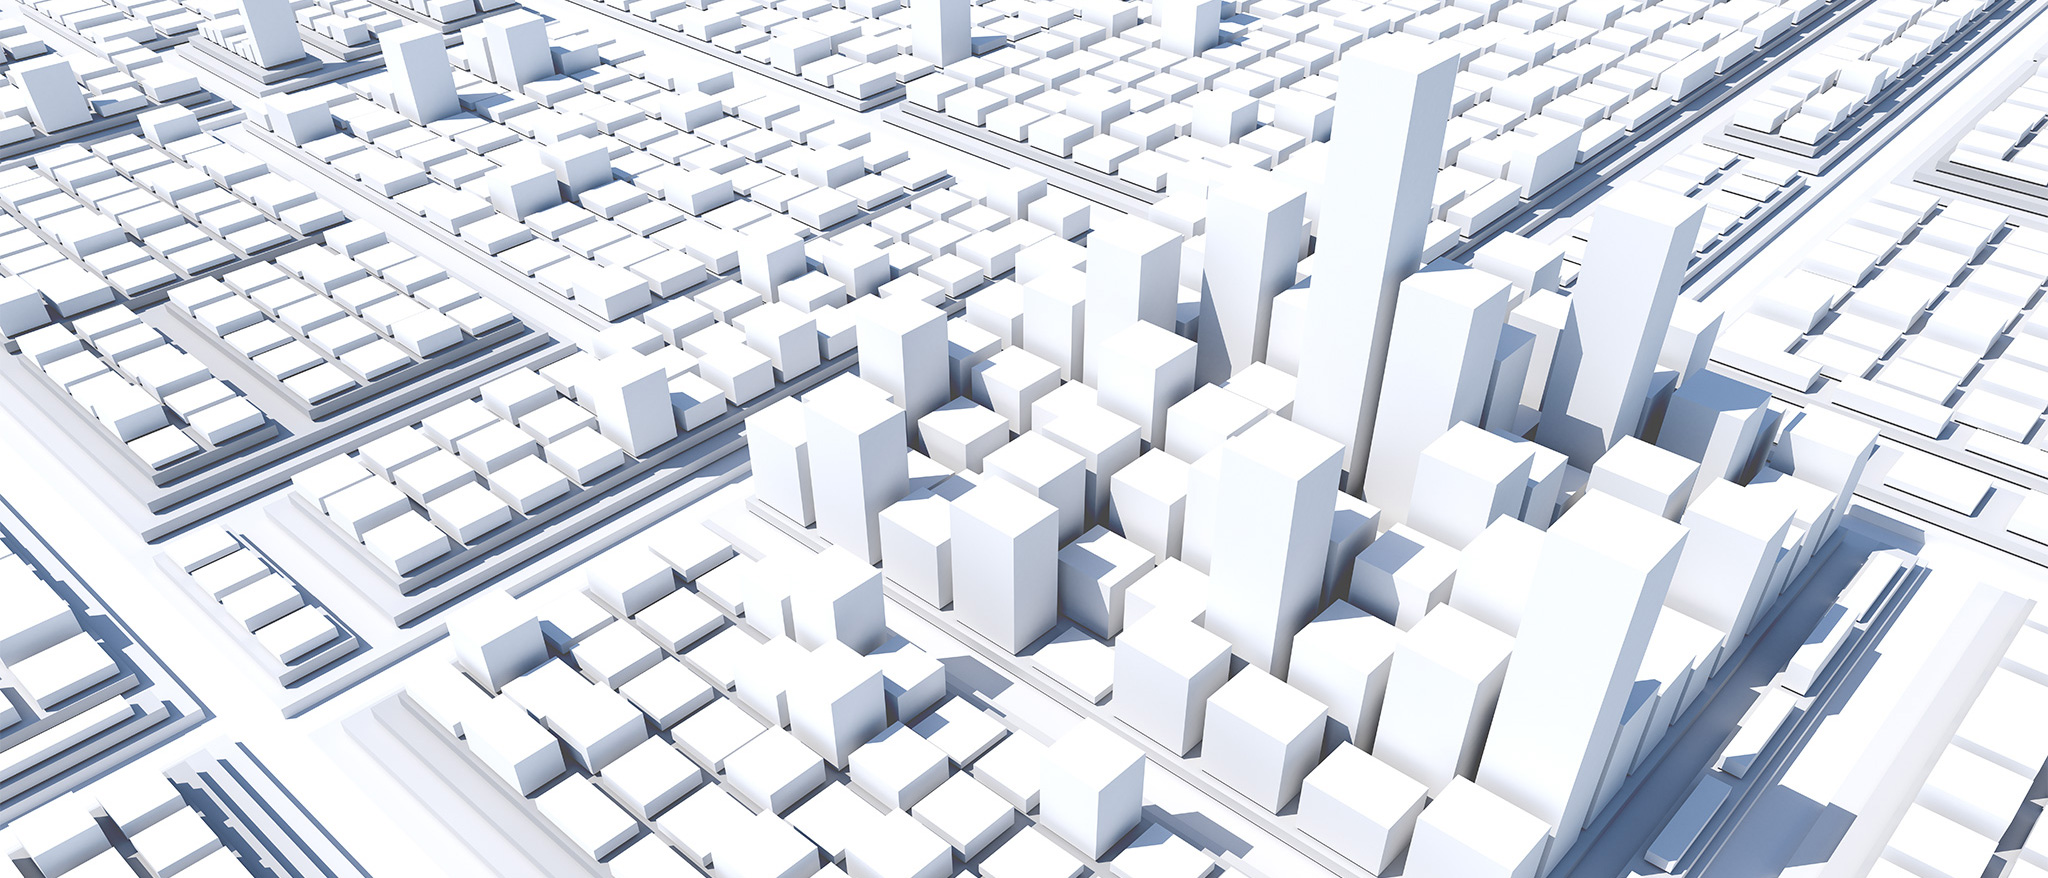
\includegraphics[width = \textwidth, clip, trim = 512 0 0 0]{figures/_white-city-map}};
    \end{tikzpicture}
    \caption{%
        An illustration of a 2.5D software map with a software metric mapped to the height of cuboids (leaf nodes) representing software modules, thus, making it a \emph{software map}. 
        Neither color nor area is used for attribute mapping. 
        Instead, it shows the expressiveness of additional visual cues, i.e., floating nodes and shadows, that can enhance the synthesized gestalt of a software system.}
    \label{fig:minimal-25d}
\end{figure*}
Treemaps denote a group of well-known, widely used, versatile techniques for visualizing information.
They enable the presentation of extensive, non-spatial, tree-structured data and reliably serve thematic maps' familiarity, convenience, and informative value.
In its most common 2D form, data is mapped to color and area. 
They can also be embedded into the third dimension, e.g., using cuboids or pyramids~\citep{turo1992-improve}, resulting in so-called 2.5D treemaps (\autoref{fig:minimal-25d}) or 3D-embedded treemaps.
These offer further possibilities for mapping and overlaying data or visual variables~\citep{carpendale2003-considering}.
2D~and~2.5D treemaps alike can support visual analytics to \enquote{foster the constructive evaluation, correction, and rapid improvement of our processes and models and---ultimately---the improvement of our knowledge and our decisions}~\citep{keim2008-visual}.
Treemaps are a tool that is used in many variations and different domains~\citep{shneiderman2009-treemaps}.
For example, they have been used to depict file systems~\citep{johnson1991-spacefilling}, stock markets~\citep{wattenberg1999-stockmarkets}, controller performance data~\citep{shah2005-controllerperformance}, health data~\citep{chazard2006-treemaps}, demographics~\citep{jern2009-choropleth}, business intelligence~\citep{vliegen2006-business,roberts2018-business}, and software development~\citep{merino2018-softvis}.
This has ultimately led to treemaps being increasingly integrated into well-known charting tools, frameworks, and libraries.

In software analytics, treemaps are used to depict software system and software engineering data, resulting in so-called \emph{software maps}~\citep{limberger2019-softwaremaps}.
Software maps are a general-purpose interactive user interface for information display in software analytics.
Typically, a catalog of \emph{software map themes} compiles commonly used attribute selections and mappings to visual variables relevant to specific tasks.
A \emph{software map theme}, hereinafter referred to as \emph{map theme}, defines a selection of software information dimensions mapped onto a software map's visual variables.
It portrays selected aspects of the software information gathered and analyzed by software analytics processes.
In a sense, a map theme presents a topic or use-case-specific software map template that supports different stakeholders in software engineering in data-driven decision-making.

To advance towards the goals of visual software analytics, i.e., \enquote{(1) derive insight from massive, dynamic, ambiguous, and often conflicting data, (2) detect the expected and discover the unexpected, (3) provide timely, defensible, and understandable assessments, [and] (4) communicate assessment effectively for action}~\citep{keim2008-visual}, we extend on the recent work of \cite{limberger2019-softwaremaps} and derive the following research questions for software maps:
\begin{itemize}
	\item How can data be depicted beyond the primary use of area, height, and color?
	\item To what extent can techniques be used individually and in combination?
	\item How does the data type impact the utilization of certain visual variables?
	\item What are helpful configurations and variations of software maps?
\end{itemize}

\begin{figure*}[t]
	\centering
	

{%
	\scriptsize
	\renewcommand{\pipelinenamesize}{\scriptsize}
    \centering
    \begin{tikzpicture}[every node/.style={inner sep=0,outer sep=0}]
    \begin{scope}[node distance = 12.25pt]
    \node [data] (problemdata) {};
    \node [phase,text width=40pt,align=center,text depth=0pt] (analysis) [right=of problemdata] {Analysis};
    \node [data] (visualizationdata) [right=of analysis] {};
    \node [phase,text width=40pt,align=center,text depth=0pt] (preprocessing) [right=of visualizationdata] {Filtering};
    \node [data] (focusdata) [right=of preprocessing] {};
    \node [smalldata] (preprocessing-config) [below=8pt of preprocessing] {};
    \node [phase,align=center] (mapping) [right=of focusdata,text depth=0pt] {Mapping};
    \node [data] (geometry) [right=of mapping] {};
    \node [smalldata] (mapping-config) [below=8pt of mapping] {};
    \node [phase,align=center,text width=40pt] (imagesynthesis) [right=of geometry,text depth=1.2\baselineskip] {Image Synthesis};
    \node [data] (image) [right=of imagesynthesis] {};
    \node [smalldata] (imagesynthesis-config) [below=8pt of imagesynthesis] {};
    \node [phase,text width=40pt,align=center,yshift=-4pt] (perception) [below=40pt of imagesynthesis,text depth=1.2\baselineskip] {Perception \& Cognition}; %
    \node [data] (knowledge) [left=of perception] {};
    \node [phase,align=center] (exploration) [left=of knowledge,text depth=0pt] {Exploration};
    \node [data] (config) [left=of exploration] {};
    \node [phase,align=center] (api) [left=of config] {API};
    \end{scope}
    \connectfromdata{problemdata}{analysis};
    \connecttodata{analysis}{visualizationdata};
    \connectfromdata{visualizationdata}{preprocessing};
    \connecttodata{preprocessing}{focusdata};
    \connectionSmallN{preprocessing-config}{preprocessing-config-center};
    \draw[draw=black,very thin] (preprocessing-config-center.center) -- (preprocessing);
    \connectfromdata{focusdata}{mapping};
    \connecttodata{mapping}{geometry};
    \connectionSmallN{mapping-config}{mapping-config-center};
    \draw[draw=black,very thin] (mapping-config-center.center) -- (mapping);
    \connectfromdata{geometry}{imagesynthesis};
    \connecttodata{imagesynthesis}{image};
    \connectionSmallN{imagesynthesis-config}{imagesynthesis-config-center};
    \draw[draw=black,very thin] (imagesynthesis-config-center.center) -- (imagesynthesis);
    \connectionS{image}{imagecenter};
    \draw[draw=black,very thin] (imagecenter.center) |- (perception) node[pos=0.75] (perceptionloop-join) {};
    \draw[draw=black,very thin] (perception.west) -- (knowledge.east);
    \connectionW{knowledge}{knowledgecenter};
    \draw[draw=black,very thin] (knowledgecenter.center) -- (exploration) node[pos=0.5] (perceptionloop-split) {};
    \draw[draw=black,very thin] (exploration.west) -- (config.east);
    \draw[draw=black,very thin,->] (perceptionloop-split.center) -- ($(perceptionloop-split)+(0pt,-16pt)$) -- ($(perceptionloop-join)+(0pt,-16pt)$) -- (perceptionloop-join.center);
    \connectionW{config}{configcenter};
    \draw[draw=black,very thin] (configcenter.center) -- (api);
    \draw[draw=black,very thin] (api) -- (preprocessing-config) node[pos=0.90] (preprocessing-config-split) {};
    \draw[draw=black,very thin] (preprocessing-config-split.center) -| (mapping-config) node[pos=0.5] (mapping-config-split) {};
    \draw[draw=black,very thin] (mapping-config-split.center) -| (imagesynthesis-config);
    \node[above=8pt of problemdata,align=center,text width=25pt,align=center] (problemdatalabel) {Problem Data};
    \draw [draw=black,very thin,shorten >= 1pt,shorten <= 2pt] (problemdata) -- (problemdatalabel);
    \node[above=8pt of visualizationdata,align=center] (visualizationdatalabel) {Visualization Data};
    \draw [draw=black,very thin,shorten >= 1pt,shorten <= 2pt] (visualizationdata) -- (visualizationdatalabel);
    \node[above=8pt of focusdata,align=center] (focusdatalabel) {Focus Data};
    \draw [draw=black,very thin,shorten >= 1pt,shorten <= 2pt] (focusdata) -- (focusdatalabel);
    \node[above=8pt of geometry,align=center,text depth=0pt] (geometrylabel) {Geometry};
    \draw [draw=black,very thin,shorten >= 1pt,shorten <= 2pt] (geometry) -- (geometrylabel);
    \node[above=8pt of image,align=center] (imagelabel) {Image};
    \draw [draw=black,very thin,shorten >= 1pt,shorten <= 2pt] (image) -- (imagelabel);
    \node[above=8pt of knowledge,align=center,text depth=0pt] (knowledgelabel) {Knowledge};
    \draw [draw=black,very thin,shorten >= 1pt,shorten <= 2pt] (knowledge) -- (knowledgelabel);
    \node[above=8pt of config,align=center,label={[xshift=-8pt,text depth=0pt]Configuration}] (configlabel) {};
    \draw [draw=black,very thin,shorten >= 1pt,shorten <= 2pt] (config) -- (configlabel);
    \begin{scope}[on background layer]
    \node [pipeline,pipelinename=Visualization Pipeline,fill=gray!8] (pipeline) [fit={($(preprocessing.north)+(0pt,2.3\baselineskip)$)(analysis.west)(imagesynthesis.east)(imagesynthesis.south)}] {};
    \node [pipeline,pipelinename=User,fill=gray!8] (user) [fit={($(exploration.north)+(0pt,2.3\baselineskip)$)(exploration.west)(perception.east)(perception.south)}] {};
    \end{scope}
    \end{tikzpicture}%
}%

	\caption{%
	    Model of the visualization process~\citep{wijk2005-visualization} consisting of a visualization pipeline~\citep{santos2004-gaining} and a feedback loop for knowledge gathering and interactive user control. 
	    This model applies to visual software analytics using software maps.}
	\label{fig:visualization-process}
\end{figure*}

To answer these questions, we discuss advanced visual metaphors and techniques for software maps by exploring the underlying visualization pipeline.
A superimposed visualization process integrates a visualization pipeline into a feedback loop with interactive user control of the various stages~\citep{wijk2005-visualization}.
Such a visualization pipeline is a sequence of three to four data processing stages with named inputs and outputs that conceptualize the transformation process of data into images.
This visualization process is well understood, and there are a few variations of models of visualization pipelines:
When using a data state reference model, the stages can be referred to as transformations, namely, (1) data transformation, (2) visualization transformation, and (3) view or visual mapping transformation~\citep{chi1998-operator,card1999-readings,chi2000-taxonomy}.
An extensive overview of specific transformations suitable for visualization purposes was provided by \cite{liu2017-advances}.
A similar naming schema uses (1) data enrichment/enhancement, (2) visualization mapping, and (3) rendering to describe the same process~\citep{haber1990-visualization}.
This schema was later refined to (1) data analysis, (2) filtering, (3) mapping, and (4) rendering~\citep{santos2004-gaining}.
We use the latter model and refer to the first two stages as \emph{preprocessing and filtering}.
\emph{Preprocessing and filtering} cover, among others, analytics, selection, enrichment, transformation, and resampling of raw data.
The \emph{mapping} stage maps abstract data to visual representations (visual variables and configuration).
Finally, \emph{rendering} creates a visual representation using image synthesis~(\cf~\autoref{fig:visualization-process}).

Using this model, we provide an overview of advanced visual metaphors that have already been or can be used in combination with software maps to approach the challenges mentioned above. %
We briefly summarize each metaphor and technique, discuss it in the context of a stage, and describe everyday practices based on our experience from research and industry projects.
We discuss the extent to which each metaphor or technique can be used to communicate different types of data and identify feasible combinations of isolated techniques and possible interferences, spanning a design space of software maps.

The remainder of this paper is structured as follows.
\hyperref[JOV:Sec:DesignSpace]{Section~\ref*{JOV:Sec:DesignSpace}} outlines the concept of software maps.
The following sections cover algorithms and techniques applied for software maps.
\hyperref[JOV:Sec:Preprocessing]{Section~\ref*{JOV:Sec:Preprocessing}} covers filtering and preprocessing techniques.
\hyperref[JOV:Sec:Layout]{Section~\ref*{JOV:Sec:Layout}} introduces layout algorithms associated with software maps.
Design decisions for mapping software data to visual primitives are discussed in \hyperref[JOV:Sec:Mapping]{Section~\ref*{JOV:Sec:Mapping}}.
The rendering-related techniques are discussed in \hyperref[JOV:Sec:Rendering]{Section~\ref*{JOV:Sec:Rendering}}.
Configuration and assembly of software maps are discussed in \hyperref[JOV:Sec:Configuration]{Section~\ref*{JOV:Sec:Configuration}}, and in \hyperref[JOV:Sec:Conclusions]{Section~\ref*{JOV:Sec:Conclusions}}, this paper concludes.

\section{Definition and Classification of Software Maps}
\label{JOV:Sec:DesignSpace}
The term \emph{software map} is not uniquely defined in software cartography. 
Each variation, such as code cities~\citep{wettel2008-large}, software cities~\citep{steinbruckner2013-evolution}, or thematic software maps~\citep{kuhn2008-thematicmaps}, focuses on their specific intended use, i.e., visualizing abundant software system and process data and, thereby, providing a communication artifact for software engineering.
\enquote{A single graphic can convey a great deal of information about various aspects of a complex software system, such as its structure, the degree of coupling and cohesion, growth patterns, defect rates, and so on}~\citep{kuhn2008-thematicmaps}.
In order to obtain a more precise, low-level definition of \emph{software maps}, we propose a definition that denotes them as a subset of treemaps using existing systematization approaches.

\cite{schulz2011-implicit} identified the following axes for the design space of implicit hierarchy visualizations: dimensionality (either 2D or 3D), node representation (graphics primitives), edge representation (inclusion, overlap, and adjacency), as well as hierarchical layout (subdivision and packing).
\cite{duebel2014-2d3drepresentation} differentiate between reference space and attribute space for a more precise classification---assuming the validity of their classification is not affected by the non-spatial nature of treemaps.
Recently, \cite{scheibel2020-treemaptaxonomy} proposed a systematization of tree visualization techniques and treemaps, including space-filling treemaps, containment treemaps, implicit edge-representation trees, and mapped trees.

\WrapFigRight{figures/_treemap-cat-s}{Space-filling treemap \Ts.}{fig:categories-space-filling}
Using these design spaces, the software map can be expressed as follows.
For the spatialization of nodes of a software map, we prefer subdivision or packing within a 2D reference space ($\mathcal{R}^2$).
\WrapFigRight{figures/_treemap-cat-c}{Containment~treemap~\Tc.}{fig:categories-containment}
The representation of edges is assumed to be implicit through nesting or inclusion, rendering a software map's underlying layout a \emph{containment treemap} layout (\autoref{fig:categories-containment} and \autoref{fig:categories-space-filling}).
Some exceptions include a layout that encodes the parent-child relationship using adjacency, resulting in \emph{implicit edge-representation trees} as software maps.
Geometric adjacency in 2.5D maps can also be used (\cf~\autoref{fig:minimal-25d}), but due to their implications with height mapping, we suggest considering its use carefully~\citep{limberger2018-filtering}; eventually, we use flat representations of inner nodes only for all map themes in order to reduce occlusion and allow for particular representation of aggregates (level-of-detail).
Techniques based on containment and overlap in 3D are marginally helpful for large data sets due to added interaction complexity and hard-to-resolve occlusion.
Fortunately, this restriction does not exclude commonly used treemap-layouting algorithms based on rectangular or polygonal shapes~\citep{hahn2017-hybrid}.
For the representation of leaf nodes, 2D graphics primitives are common, e.g., Voronoi shapes or rectangles ($\mathcal{A}^2$).
Embedded in 3D, they can be extruded, optionally tapered, and thus use the third spatial dimension ($\mathcal{A}^3$).
\enquote{Increasing the visual vocabulary can provide for richer information resolution}~\citep{turo1992-improve} and allow for additional information display.
For these 2.5D software maps, we generally prefer graphical primitives of rectangular footprints over more complex ones (\cf~\hyperref[fig:complex-examples]{\autoref*{fig:complex-examples} (a)})---depending on (1) the importance of stability for the respective map theme and (2) whether or not rendering of more complex geometry is justifiable in terms of visual complexity, implementation complexity, as well as interactivity and responsiveness of the visualization.
Since the reference space is still in $\mathcal{R}^2$, we support the terms \emph{2.5D}~\citep{turo1992-improve} and \emph{3D-embedded} to avoid confusion with actual 3D~treemaps that use 3D~layouts for positioning graphical elements in a 3D~reference space ($\mathcal{R}^3$).

With the attribute space and reference space being constrained, the typical characteristics of $\mathcal{A}^2\otimes\mathcal{R}^2$ and $\mathcal{A}^3\otimes\mathcal{R}^2$ visualizations adhere to software maps.
Consequently, we define software maps as a subset of 2D and 2.5D containment treemaps---with some exceptions being implicit edge representation trees---for the targeted mapping of abstract software system data and software engineering data as well as software development data.
This gives one outstanding benefit: their characteristics largely match those of ubiquitously available, interactive 2D and 2.5D (geo-spatial) maps.
Furthermore, with this definition of software maps, both visualization engineers and software engineers can rely on and build upon familiar (1) interaction metaphors, (2) provisioning strategies, and (3) visualization metaphors, drawing on their habits and experiences.

\subsection{Data Characteristics}
Traditionally, visualizations targeting software analytics are required to handle three essential aspects of software system data: static, dynamic, and evolving aspects~\citep{diehl2007-software}.
We use a broader scope for software maps by including software development data and all stakeholders of the software development process.
The data typically covers mined, preprocessed data gathered from various sources:
\begin{itemize}
	\item Software implementations: typically modularized, available as distributed tree-structured components and source code units. In addition to topology information, metrics and other \emph{key performance indicators} (KPIs) are measured and derived by applying static source code analysis to the programmed artifacts, namely source code, scripts, binaries, and documentation.
	\item Software executions (\emph{traces}): e.g., analysis of run-time execution to capture and measure a software's behavior.
	\item Software development processes and evolution: e.g., analysis of the engineering work on the system done by software developers. This data is usually available in revisioning systems and issue, bug, and customer feedback tracking tools.
\end{itemize}

Even if measured precisely, the data is (1) prone to uncertainty, (2) vague semantic normalization, (3) lacks standardized metrics and interpretations, and (4) is highly language-specific and, thus, highly heterogeneous in large software systems.
Furthermore, anonymization may be required, the resolution of measurements is unnecessarily high, and the data quickly becomes extremely extensive and complex even for medium-sized projects (metrics per file and per commit, every change with respect to issue tracking, continuous integration).
These characteristics should be considered when specifying map themes or developing visualization techniques for visual information display using software maps.
An overview of visualization techniques for static aspects and their evolution, including visualization techniques besides treemaps and software maps, is listed in surveys by \cite{caserta2011-staticaspects} and \cite{merino2016-actionable}.

\subsection{Preliminaries and Assumptions}
This paper does not provide a comprehensive set of design guidelines for creating treemaps regarding all aspects of visualization design.
Guidelines concerned with perception~\citep{kong2010-guidelines} or use of color~\citep{xie2017-coloraesthetics,schloss2018-colormap,quinan2019-discretization} are not specific to treemaps but relevant for every visualization and, thus, not the focus of this paper.
Especially for color, we suggest referring to geographic, thematic maps and commonly used, sequential, diverging, and qualitative color schemes.

\WrapFigRight{figures/_visual-clutter-cropped}{Depiction of a software system with hundreds of thousands of software artifacts.}{fig:clutter}
Our selection of discussed visualization techniques focuses on metaphors and techniques that cope with the data characteristics within software engineering, i.e., volume and complexity of the data (\autoref{fig:clutter}).
Therefore, we prefer techniques that have already been introduced for software data and can handle data sets with lots of data elements.
Similarly, we focus on visualization techniques that entail abstract depictions, i.e., we follow the approach of mapping abstract software data---data without any natural \emph{gestalt}---to abstract visual entities.
This paper does not cover city visualizations or city-like metaphors~\citep{knight1999-comprehension,balogh2015-codemetropolis} that map abstract data to features of virtual 3D cities such as building facades, car or pedestrian traffic, or street furniture.

\subsection{Software Maps and Landscapes}
\begin{figure}[t]
    \centering
    \begin{tikzpicture}[figNS, spy using outlines = {style = { spyRC, spypink }, magnification = 4.0, size = 34mm}]
        \node[figRC, anchor = east](fig0) at (0,0)
            {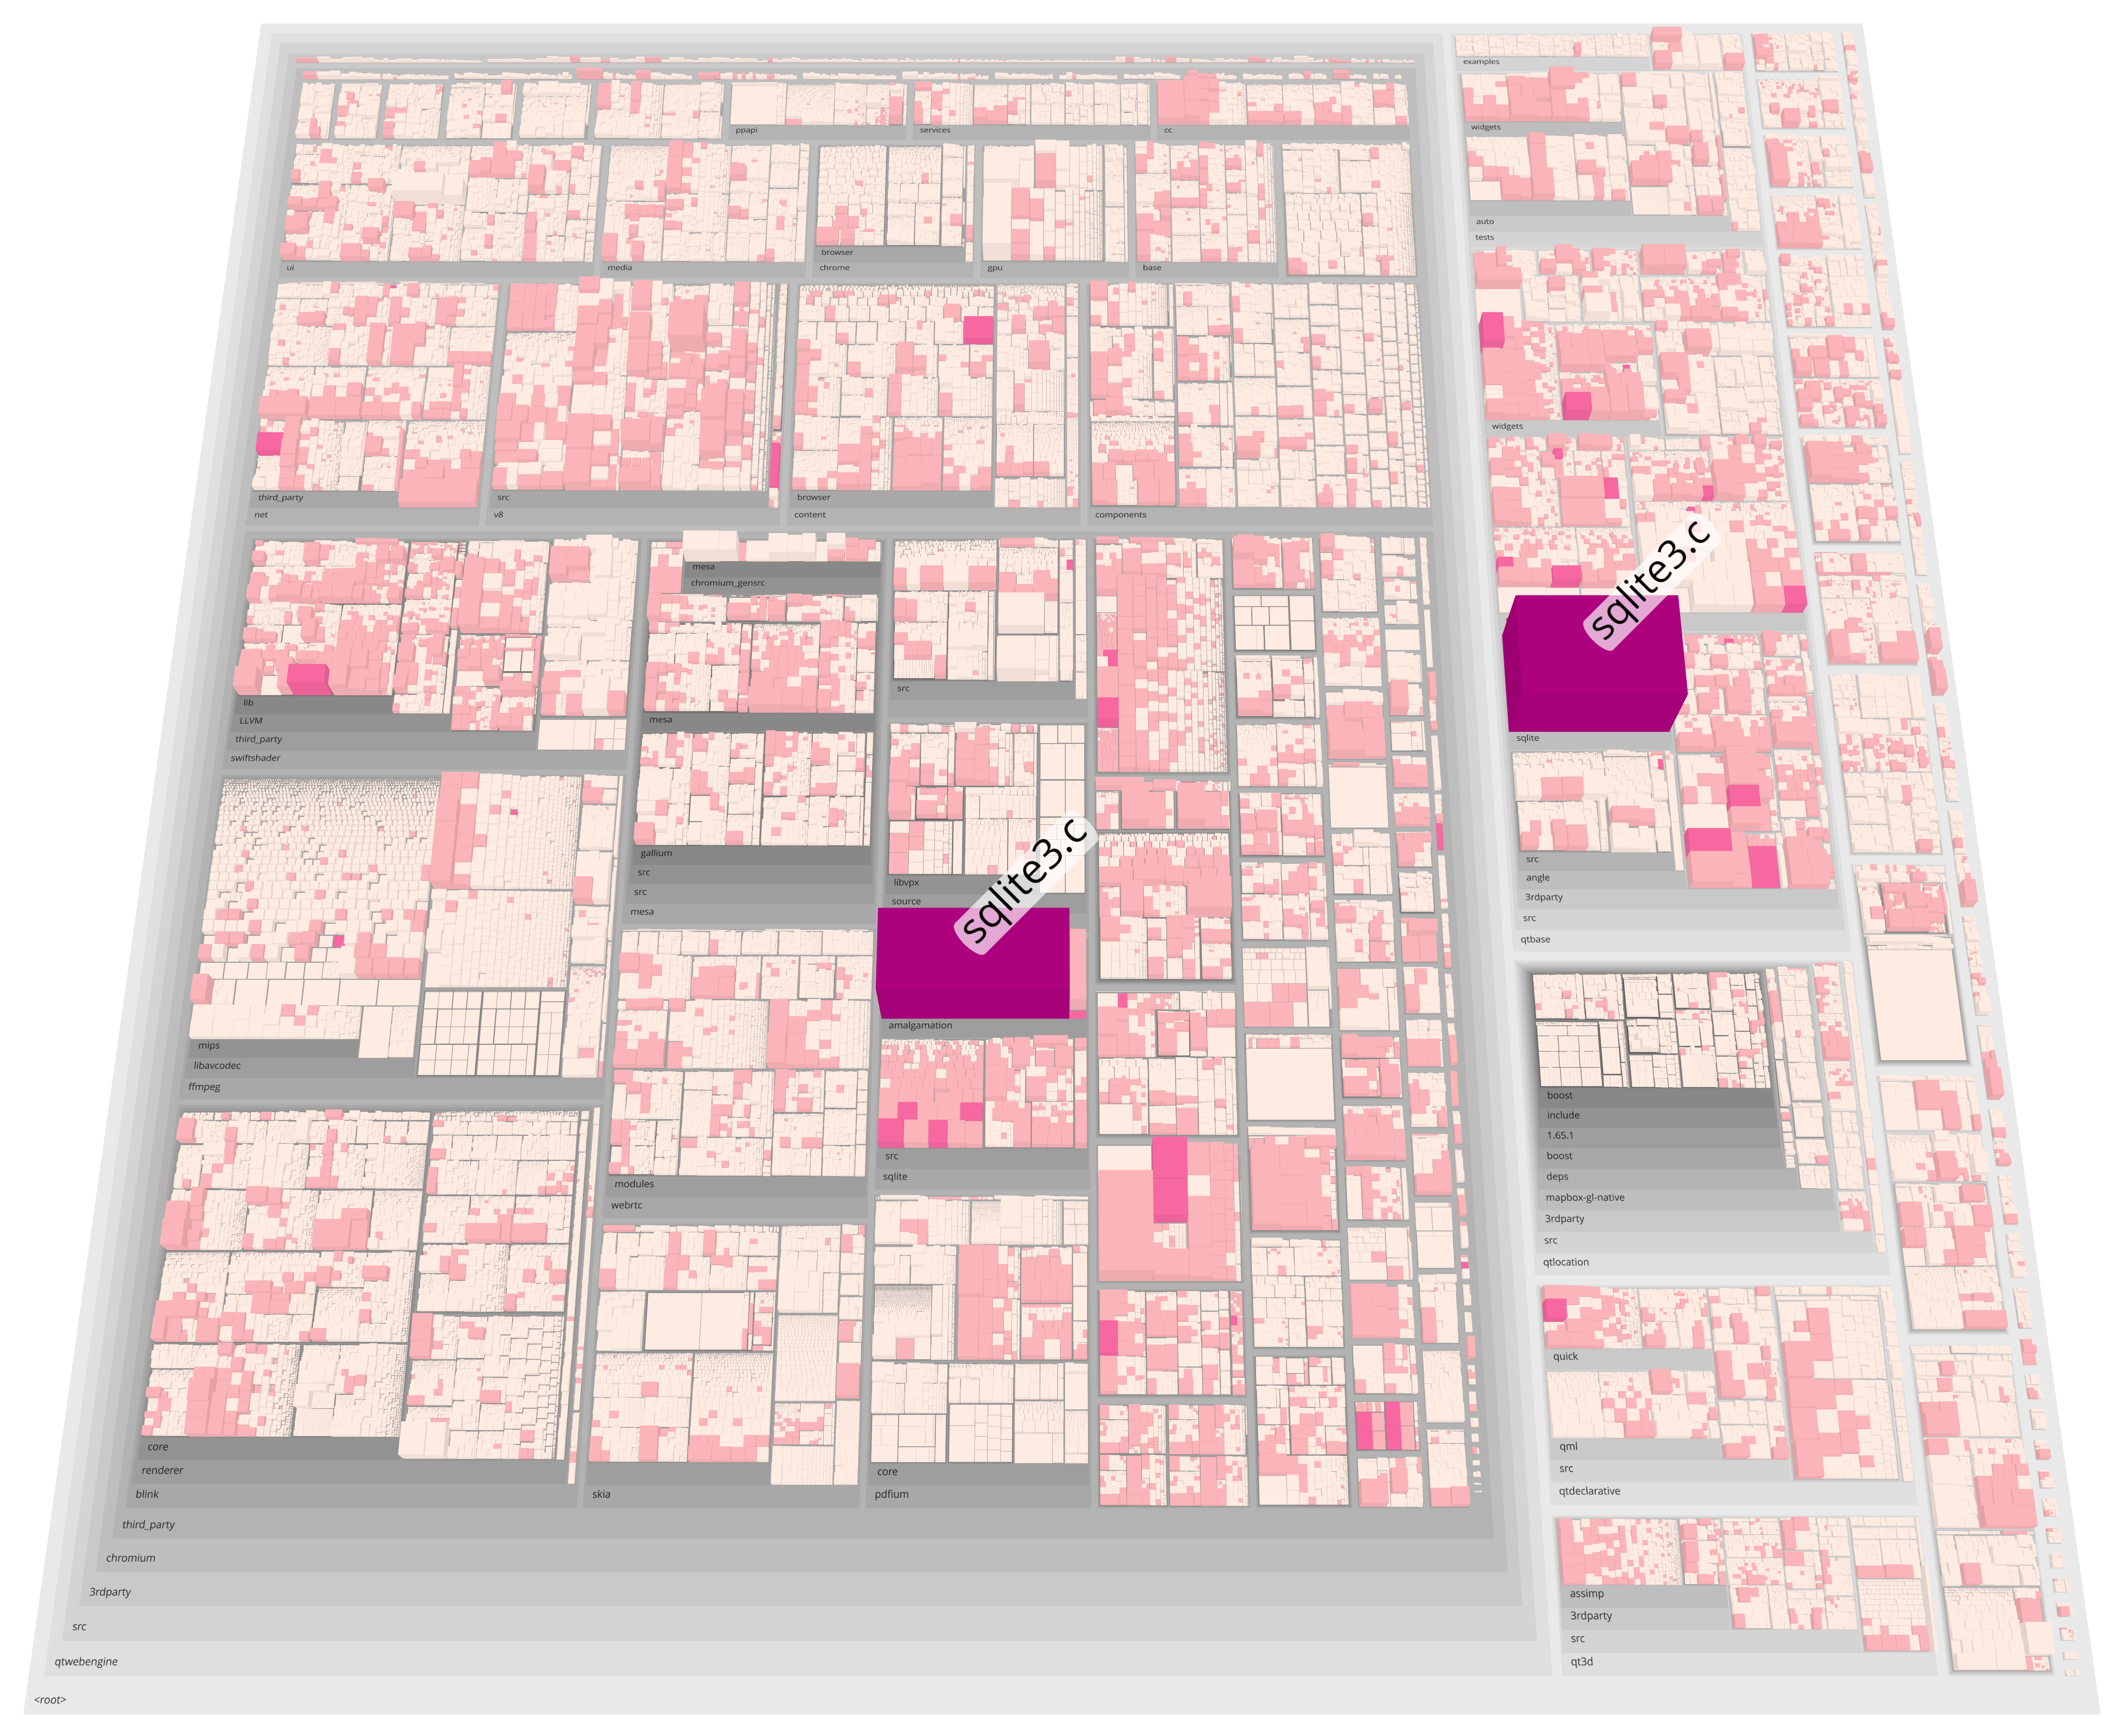
\includegraphics[width = 0.71\linewidth, trim = 64 96 64 32, clip]{figures/qt-software-map.png}};
        \spy on ($(fig0.east)+(-22mm, +29.50mm)$) in node at ($(fig0.east)+(+18mm,+18mm)$);
        \spy on ($(fig0.east)+(-18mm, -29.75mm)$) in node at ($(fig0.east)+(+18mm,-18mm)$);
    \end{tikzpicture}%
    \caption{%
        A software map depicting the source code of the Qt 5.2.1 release in 2014. 
        The map contains over \numprint{145000} leaf nodes and covers most dependencies such as sqlite3 and assimp. 
        The software data was extracted from the GitHub mirror \href{https://github.com/qt/qt5}{github.com/qt/qt5} with resolved submodules.}
    \label{fig:qt-software-map}
\end{figure}
As one example of a software project, the Qt 5.2.1 release from February 2014 concluded over 19 years of development from over \numprint{1400} developers that created more than \numprint{120000} commits.
The entire functionality is distributed over more than \numprint{145000} source files with over \numprint{21000000} lines of code~(\autoref{fig:qt-software-map}).
We see this project as a large-sized software project, typical in industry contexts and, for now, widely used open-source software.
Although Qt contains various dependencies within its source code, the more recent approach would be to use software packages, which hide a large part of the source code relevant when working on projects.
Much of the source code is present in today's software through dependency on software packages.
This is important to keep in mind when exploring metrics using software maps.
Software maps and, generally, most depictions based on a software's underlying hierarchy or structure tend to obfuscate a software's overall complexity since they only cover its top-most layer. 
The dependency tree of an NPM package, for example, has an average depth of 4.39 and a size of 86.55~\citep{vaidya2019-npm-security}.
This quickly results in tens of thousands of additional source and configuration files (i.e., located in the node\_modules directory) that are usually not incorporated in the software analysis.

Whether it is more or less adequate to focus on a slice of software or cover all of it depends on the task and needs to be researched in more detail.
Extending the idea of software maps to a \emph{Google-Earth}-like service to explore millions of software projects as a landscape, planet, or galaxy is tempting.
From an implementation perspective, available frameworks and tools need to scale to large and massive datasets.
This includes preprocessing and layouting~\citep{scheibel2021-hilbertmooreperformance}, hardware-accelerated rendering, and dynamic updates of the geometry~\citep{trapp2013-gputreemaps,scheibel2016-avcs}.
Similarly, the deployment and provisioning of data and visualization are domain- and application-specific~\citep{limberger2013-interactive,limberger2016-declarative3d}.
However, a generalized view of application scenarios allows deriving common characteristics and shared approaches for visualization, including visualization services~\citep{scheibel2020-modular-hiviser}.
Based on these techniques, the foundations for a scalable and much more comprehensive exploration already exist.
For the following techniques in the phases of preprocessing, layouting, mapping, and rendering, implementations should focus on scalability.

\section{Preprocessing and Filtering}
\label{JOV:Sec:Preprocessing}
The incoming data, also known as the problem or task data, is transformed and prepared for visualization during preprocessing and filtering.
This includes resampling, normalization, filtering outliers, and accumulating weighted leaf-node data to inner nodes.
The main goal is to prepare use-case-specific data augmentation, value resolution, and data residence.
The latter two are essential for visualization systems that process large amounts of data.

\subsection{Use-case-specific Handling of Data}
Typical tasks for preparing the data for visualization result from the requirements of the visualization techniques used or the use case at hand.
Prevalent examples are area mapping in treemap layouting algorithms where a value of an inner node is expected to be the sum of all children's weights~\citep{johnson1991-spacefilling} and mapping of additional visual variables on inner nodes to display aggregated information~\citep{limberger2017-aggregation}.
When dealing with data entailing uncertainty, the aggregation of values should employ an uncertainty model~\citep{gortler2017-bubbletreemaps}.
Especially for values that are used for area mapping, there are additional techniques to manipulate the values, e.g., to allow for (1) user-controlled sizes~\citep{turo1994-basketball}, (2) scaling of otherwise invisible nodes~\citep{csallner2003-diversification}, (3) equalization of size through \enquote{atrophication}~\citep{bladh2004-threedimensions}, (4) employing a degree-of-interest~\citep{schlechtweg2004-interactive}, and (5) pre-allocating weights for the display of inner nodes~\citep{yang2015-cabinettree}.

Another example is the preprocessing of tree-structured topology.
A common approach is to process the topology through the filtering of nodes.
This reduces the display of information, selecting relevant subtrees and omitting irrelevant nodes~\citep{veras2017-minimumdescription,limberger2017-aggregation}, e.g., detection and removal of source code duplicates, generated code, automated activities, and filtering of irrelevant areas such as third-party code.
For the particular case of inner nodes having an inner node as a single child, tree pruning can be applied to simplify the topology~\citep{bladh2004-threedimensions}.

\subsection{Value Resolution}
While assembling software maps in practice, we encountered several challenges.
These include handling large amounts of data and ensuring reasonable memory usage in both main and graphics memory.
Fortunately, the required data resolution for the visualization is usually much lower than the resolution of the input data.
In these cases, we suggest reducing the data to a resolution appropriate for the map theme, e.g., attributes mapped to area, color, or height do not require a 32-bit floating-point resolution.
Often, a reduction of attribute resolution to a few bits can increase readability by means of discriminability and emphasize the results of the preceding data analysis.
This can also be supported from a perceptual point of view: height with perspective foreshortening is hardly comparable on a per-pixel basis.
The exact size of a module within a software map should be of subordinate importance.
Thus, most often, a transformation to a categorical data type such as \emph{irrelevant}, \emph{low}, \emph{medium}, and \emph{high} (for color, height, or change) or \emph{lower-outlier}, \emph{below average}, \emph{average}, \emph{above average}, and \emph{upper-outlier} (for area) are easily comparable and more effective~\citep{wettel2007-comprehension}.

\subsection{Streaming and Level-of-Detail}
The major challenge is that industry software projects tend to be massive in terms of the number of modules, code units, metrics, or activities.
This is often ignored or only marginally covered in research but significantly impacts visualization design and software map assembly.
Software maps are likely to be streamed on-demand (e.g., node by node, slice by slice).
Loading millions of attribute values for nodes that should not even be depicted, e.g., as they are out of scope or sub-pixel size, can decrease responsiveness and result in visual clutter or memory shortages.
It is advantageous to have a customizable, interactive level-of-detail~\citep{elmqvist2010-aggregation,limberger2017-aggregation} in both filtering and rendering that allows for dynamic detail (\cf~\autoref{fig:stepwiseaggregation}).
Furthermore, the software map should always support the concept of mental maps~\citep{liu2010-mentalmodels}, i.e., the overall layout should not change due to a dynamic level of detail.
\begin{figure*}[t] %
    \begin{tikzpicture}[figNS, spy using outlines = {style = spyRC, magnification = 2.5, width = 24mm, height = 20mm}]
        \node[figRC, anchor = west](fig1) at (0, 0) %
            {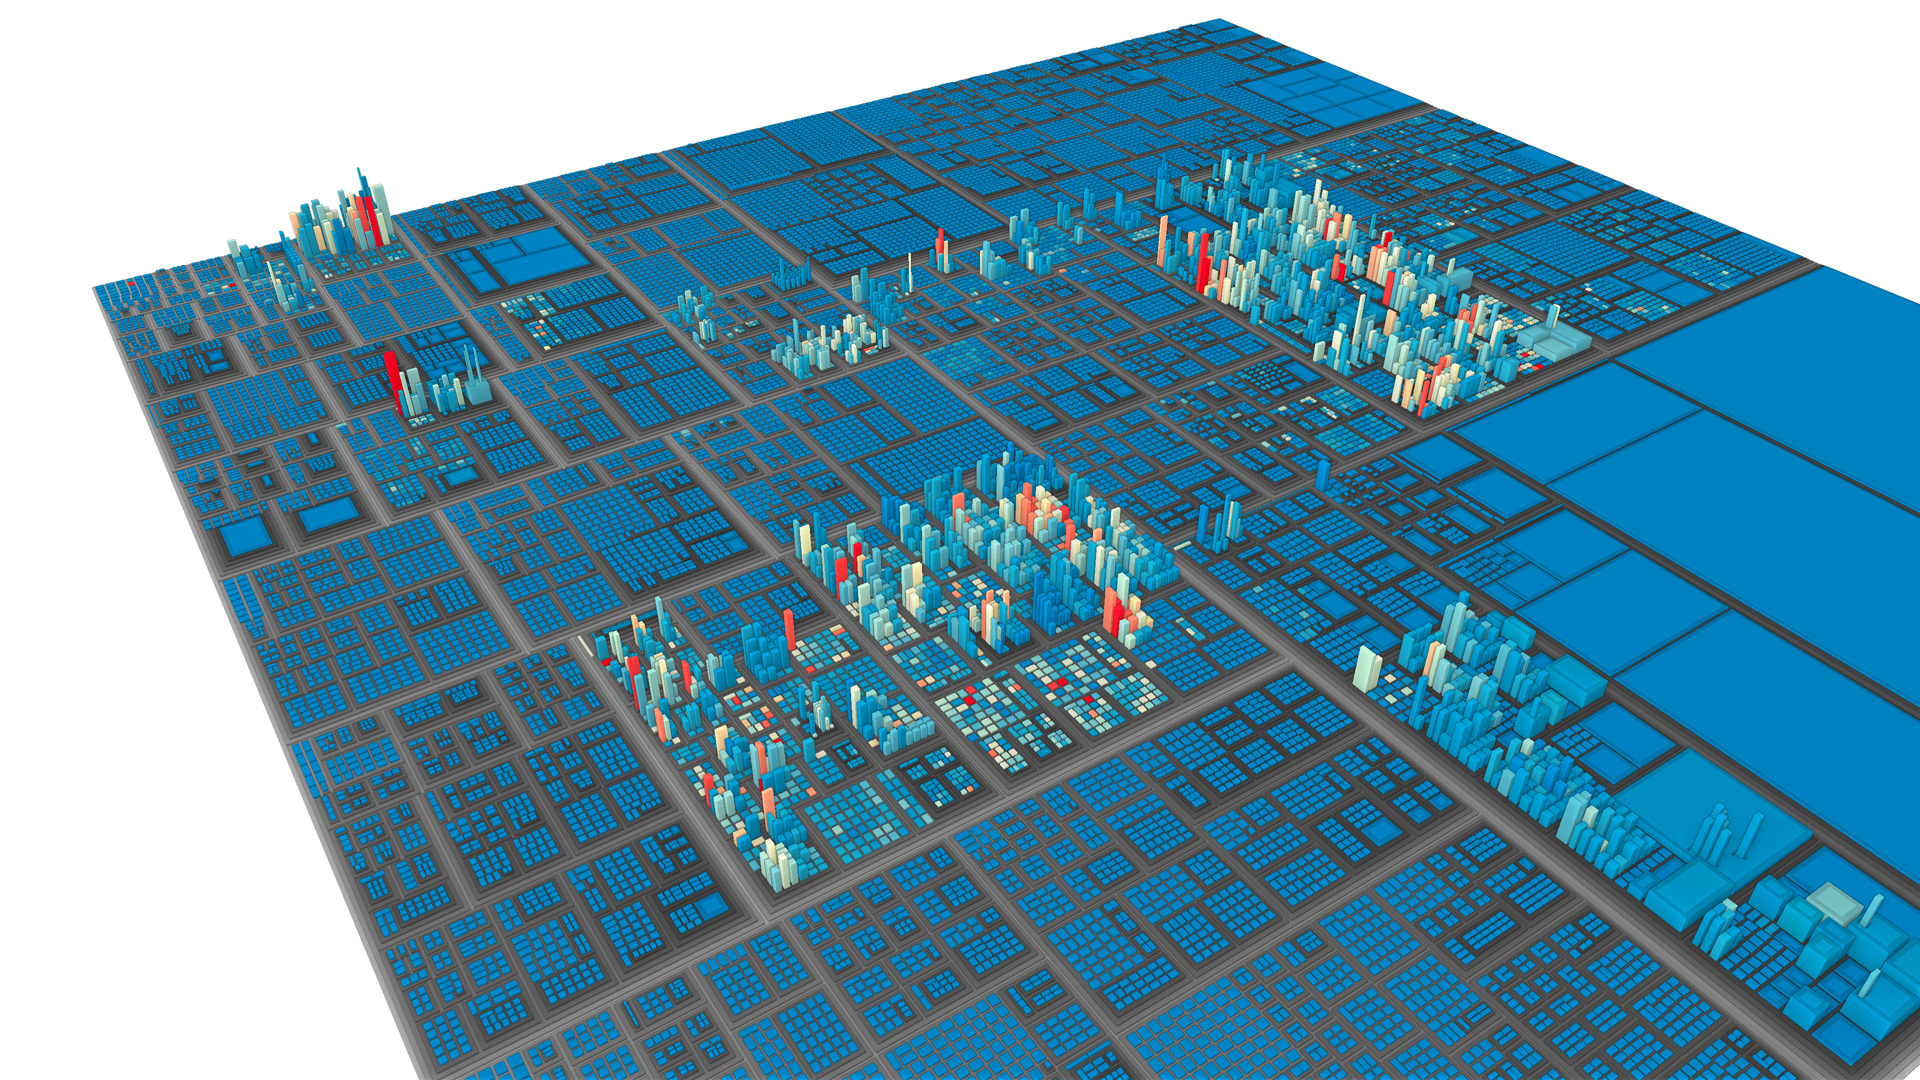
\includegraphics[width = \twffffp, trim = 704 256 704 64, clip]{figures/_aggregation-with-outlier-1}};
        \node[figRC, anchor = west](fig2) at ([xshift = \pfull] fig1.east) 
            {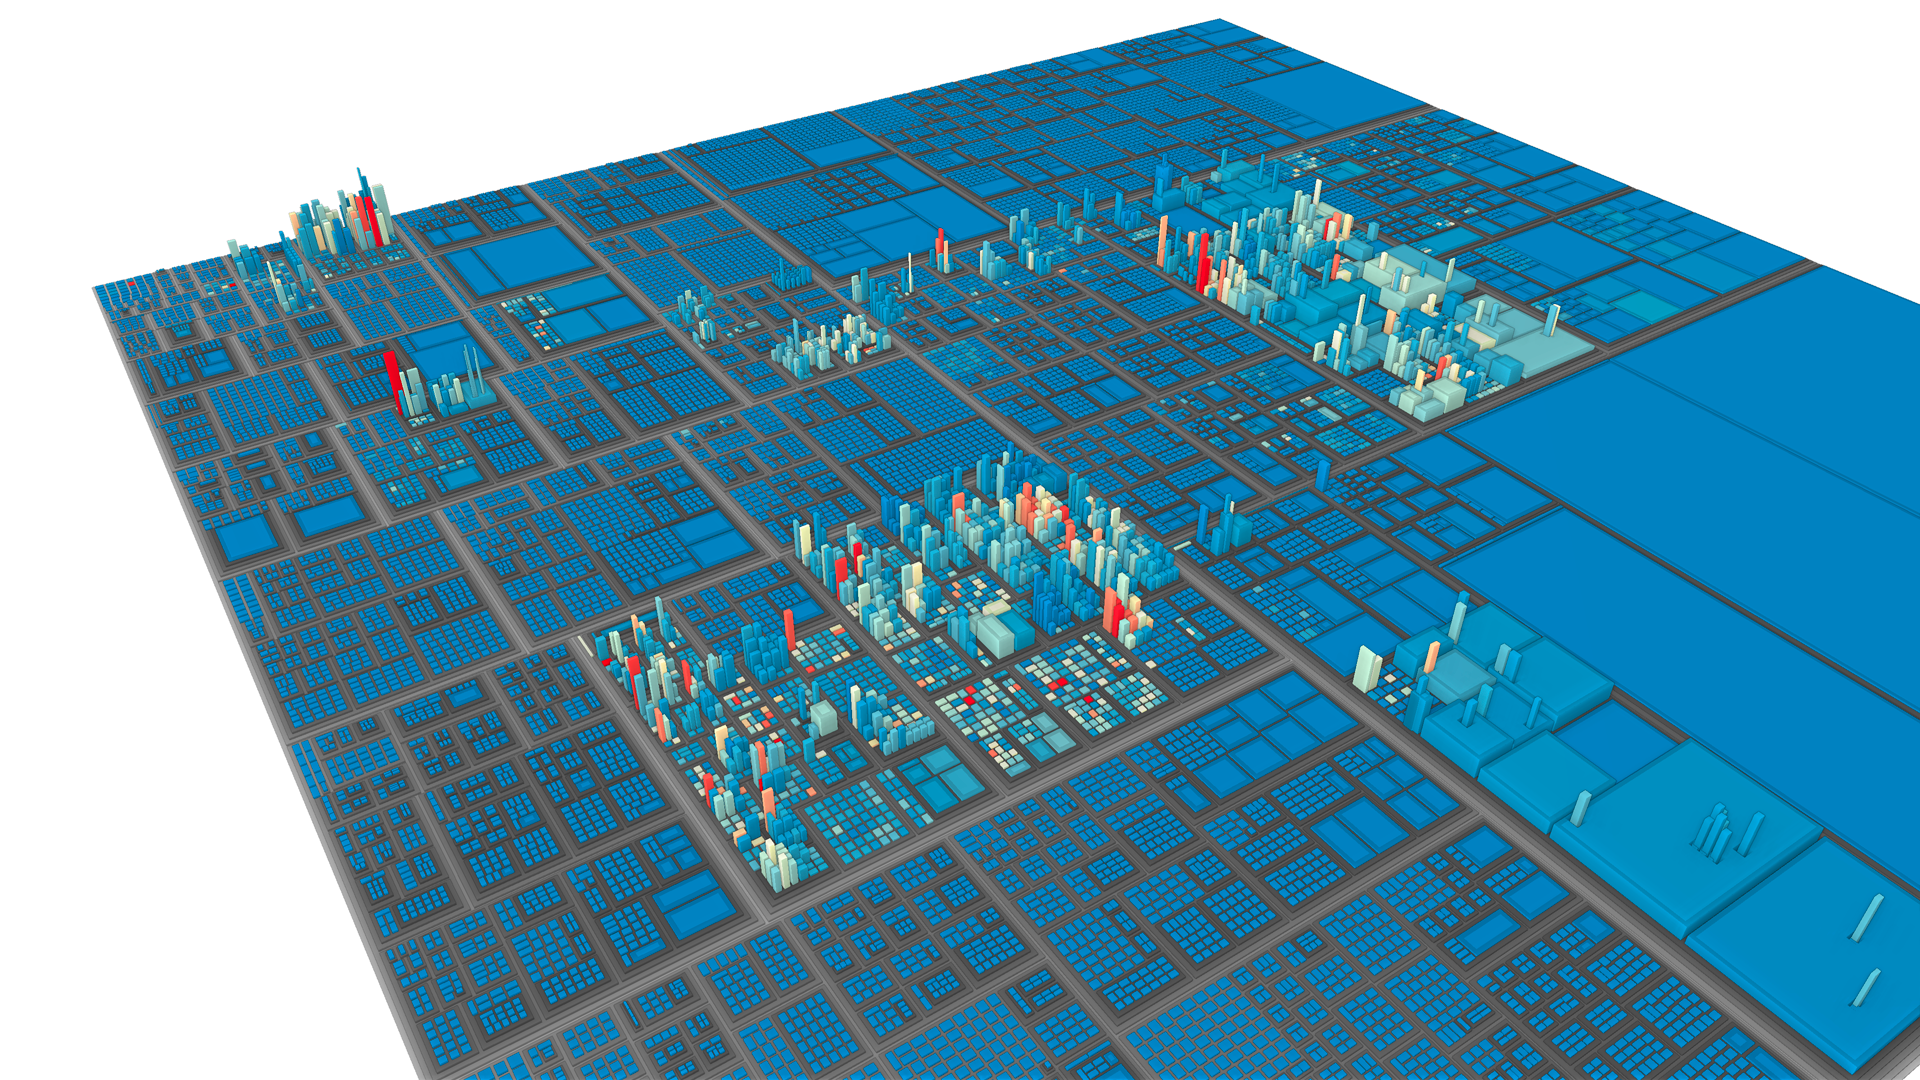
\includegraphics[width = \twffffp, trim = 704 256 704 64, clip]{figures/_aggregation-with-outlier-2}};
        \node[figRC, anchor = west](fig3) at ([xshift = \pfull] fig2.east) 
            {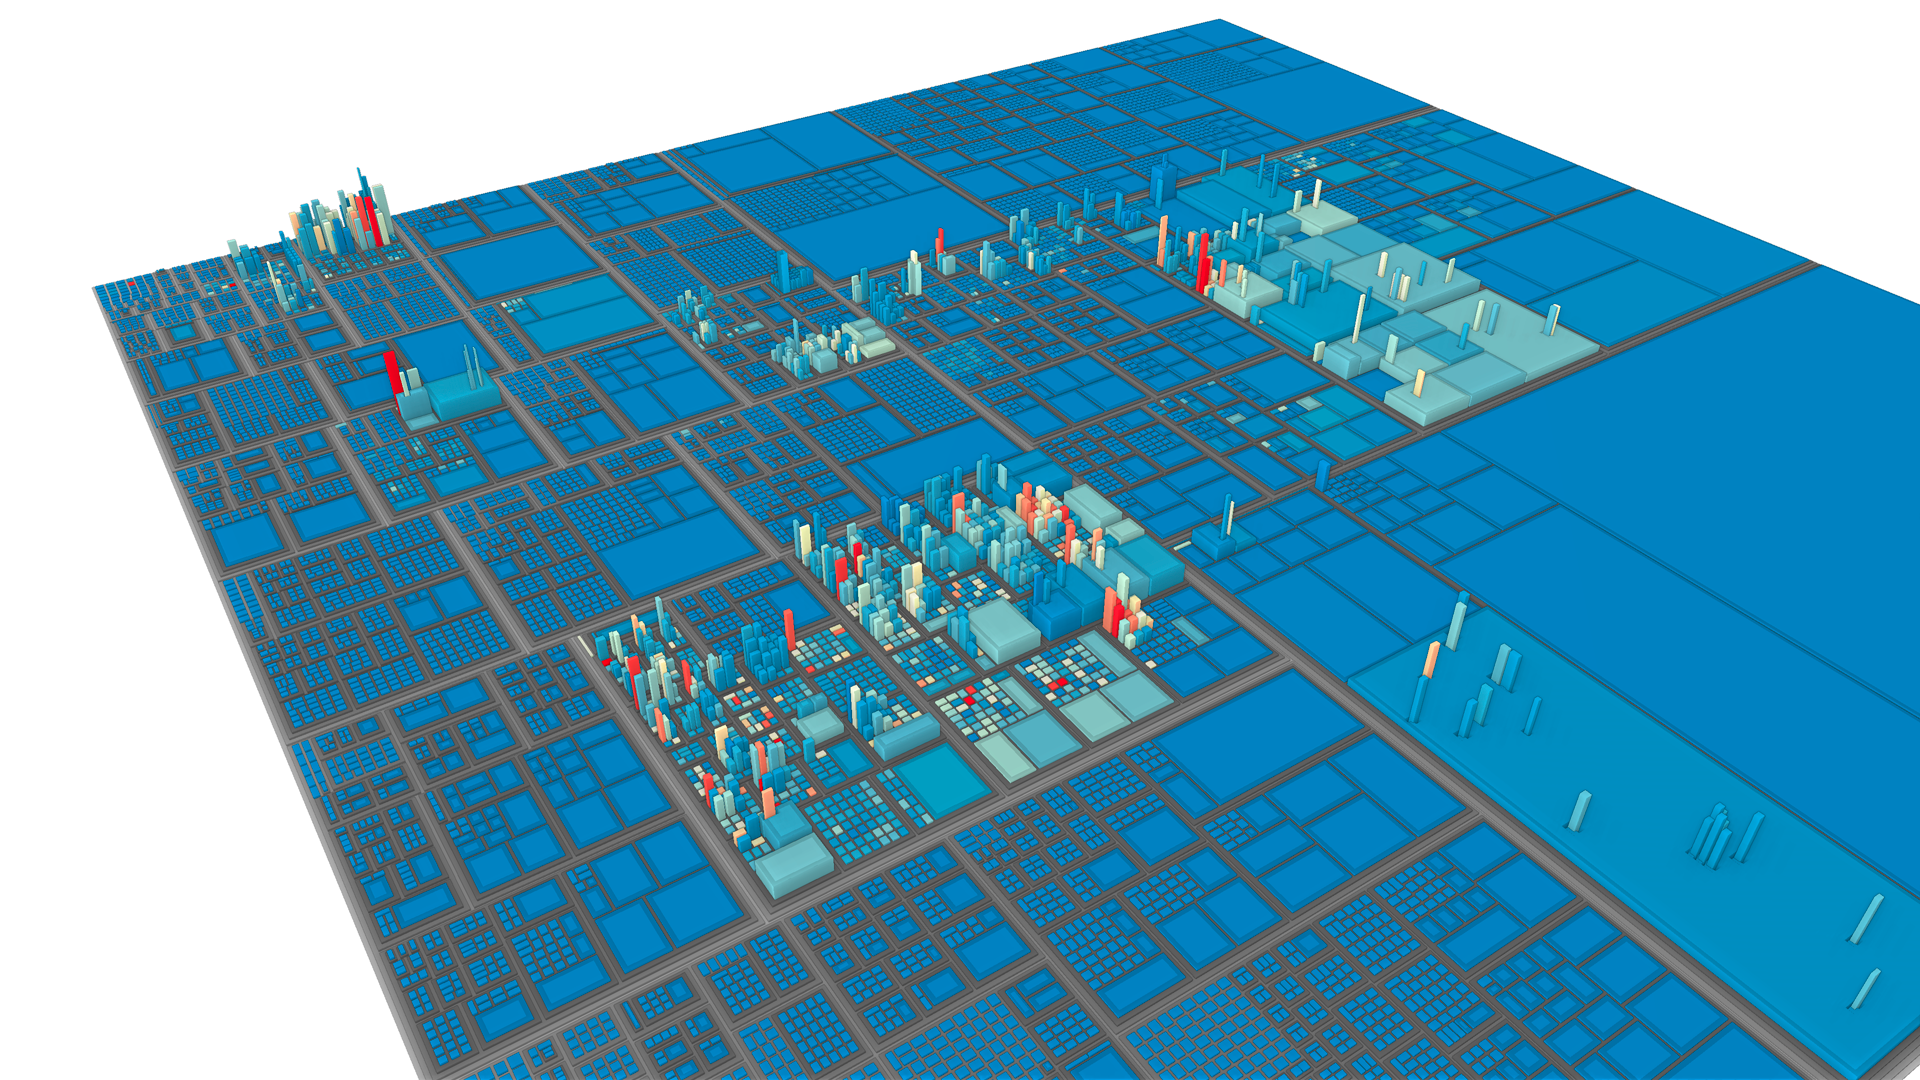
\includegraphics[width = \twffffp, trim = 704 256 704 64, clip]{figures/_aggregation-with-outlier-3}};
        \node[figRC, anchor = west](fig4) at ([xshift = \pfull] fig3.east) 
            {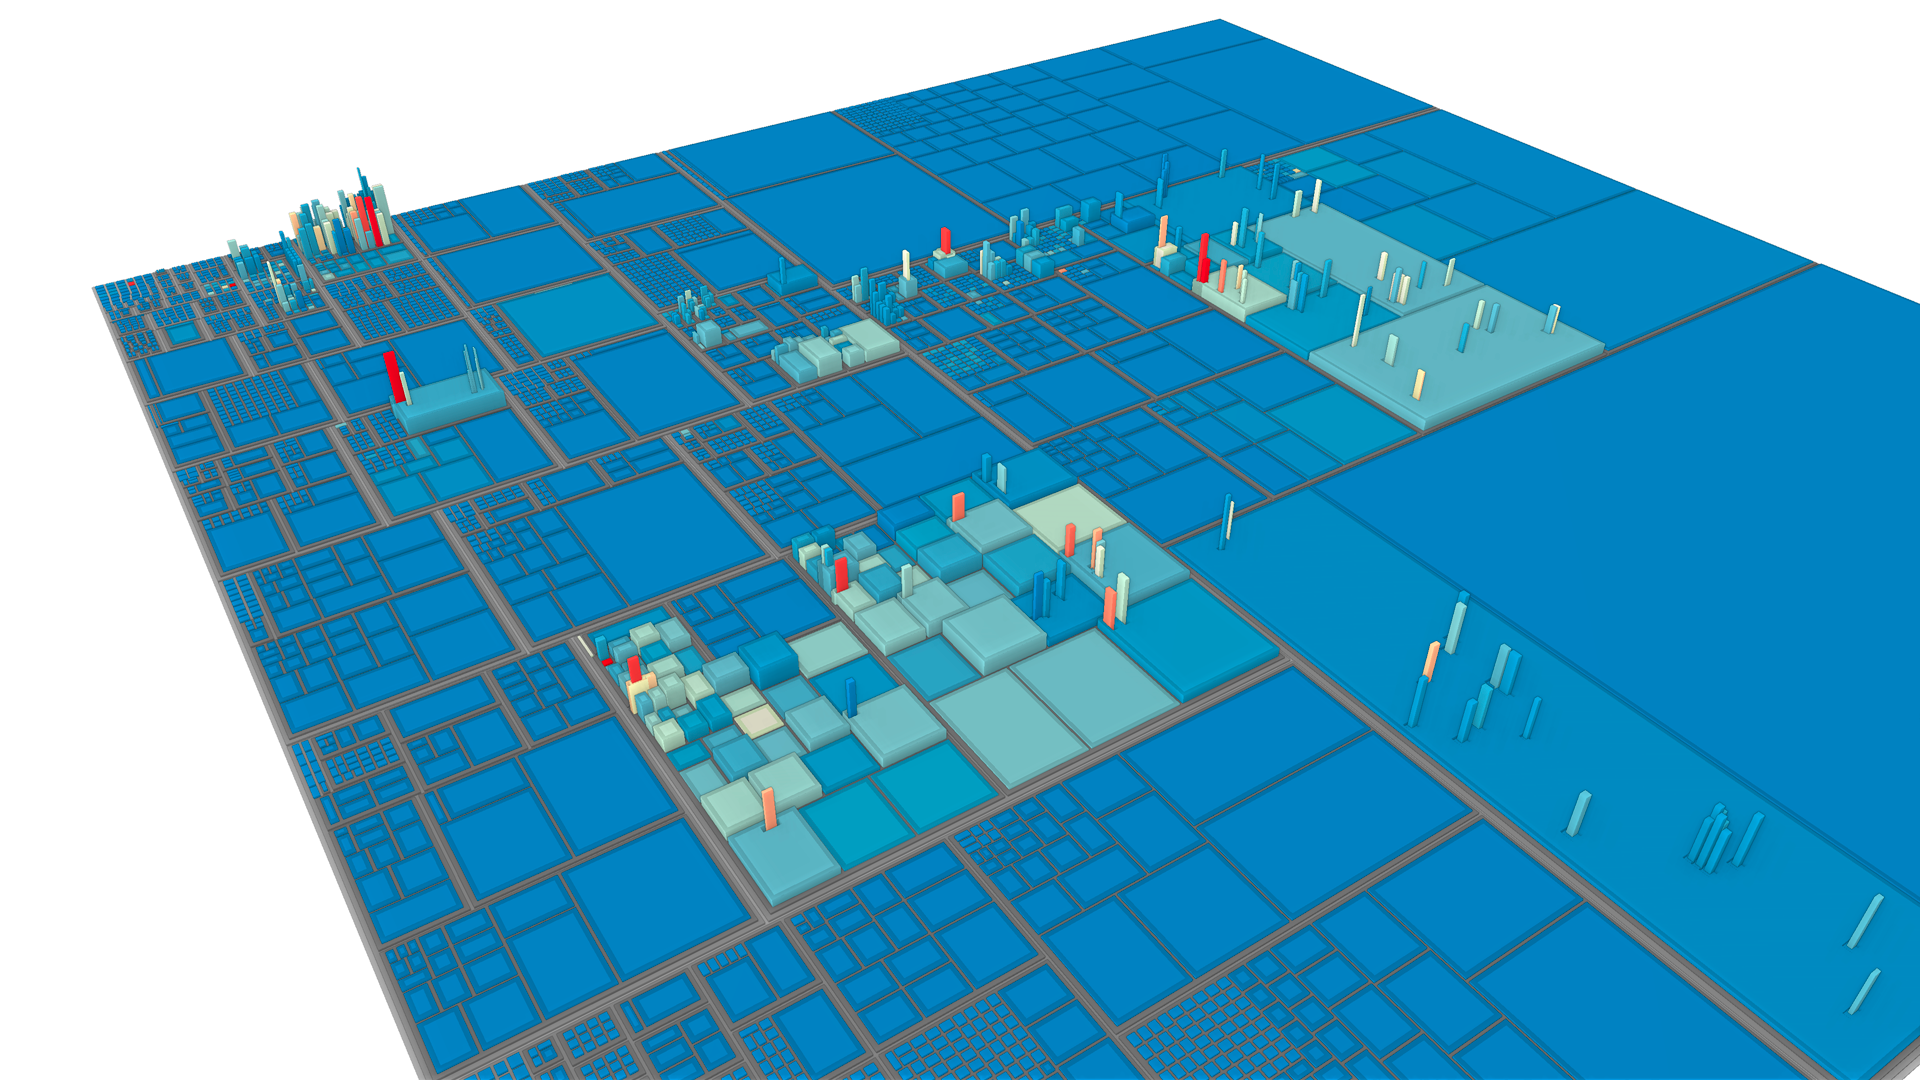
\includegraphics[width = \twffffp, trim = 704 256 704 64, clip]{figures/_aggregation-with-outlier-4}};
        \node[below left = 0 of fig1, labelSW](lab1){(a)};
        \node[below left = 0 of fig2, labelSW](lab1){(b)};
        \node[below left = 0 of fig3, labelSW](lab1){(c)};
        \node[below left = 0 of fig4, labelSW](lab1){(d)};
        \spy on ($(fig1.center)+(2mm, -3mm)$) in node at ($(fig1.north)+(0mm,-9mm)$);
        \spy on ($(fig2.center)+(2mm, -3mm)$) in node at ($(fig2.north)+(0mm,-9mm)$);
        \spy on ($(fig3.center)+(2mm, -3mm)$) in node at ($(fig3.north)+(0mm,-9mm)$);
        \spy on ($(fig4.center)+(2mm, -3mm)$) in node at ($(fig4.north)+(0mm,-9mm)$);
    \end{tikzpicture}
    \caption{%
        Stepwise simplification of a software map using aggregation, ranging from no aggregation (left) to strong aggregation (right).
        The level of aggregation can be controlled using nodes of interest or, as shown here, based on the tree level.
 		Note that outlier nodes, so-called landmarks, are preserved~\citep{limberger2017-aggregation}.}
    \label{fig:stepwiseaggregation}
\end{figure*}

\section{Layout}
\label{JOV:Sec:Layout}
The base layout for a software map can, for example, be derived from the hierarchical structure of the software project that is captured in a tree-structured dataset.
Software maps usually use inner nodes to depict applications, modules, or source code units, i.e., source code files.
The leaf nodes depict modules, source code units, functions, events, developers, activity through commits, or associated data~\citep{ardigo2021-datamaps}.
The position of each node is computed by a layout technique specified by the map theme, and a metric is mapped to the size of the graphical primitive, e.g., lines-of-code or file size.
This hierarchical structure is processed by treemap layout algorithms, resulting in treemap layouts.

\paragraph{Treemap Layout Algorithms for Software Maps.}
There are many algorithms available and under current research~\citep{scheibel2020-treemap-layout-algorithms}.
From them, mainly two-dimensional layouts are used for both 2D and 2.5D software maps.
As a prominent classification, \enquote{one can discern two major layout methodologies: \emph{subdivision} and \emph{packing}}~\citep{schulz2011-implicit}.
\emph{Packing layouts} use a spatial arrangement of child nodes based on proximity and the definition of an enclosing space as a separate layout.
\emph{Splitting layouts}, in contrast, define a space for the root node and dissect its layout for all of its child nodes.
Another approach to differentiation is the class of shapes and metaphor for hierarchical nesting that an algorithm selects for the nodes.
We see the coarse categories of rectangular splitting layouts, rectangular packing layouts, polygonal layouts, and adjacency layouts for software maps.
\WrapFigRight{figures/_splitting-layout}{Mixed splitting layout for software maps including rectangular and polygonal shapes.}{fig:mixed-layout}

\paragraph{Choice of Software Map Layout Algorithms.}
The choice of a layout algorithm for a software map may depend on several factors and goals~(\autoref{fig:mixed-layout}).
For example, the resulting whitespace can be the target for reduction, create more compact software maps, create and maintain landmarks, or as space for flexibility during layouting, e.g., allow for later insertions of nodes.
The treemap layouts are a target for general optimization for treemap layout metrics~\citep{vernier2020-quantitativecomparison}.
However, the one main parameter is the choice of the leaf node type, as it dramatically influences the metaphor and general look of the software map.
This results in software maps using either strict structures (space-filling rectangular layouts) or uniform leaf node shapes (packing layouts).
The choice of algorithms and, thus, an underlying layout parameterization allow for different metaphors for the resulting visualization.

\subsection{Rectangular Splitting Layouts}
\WrapFigRightRaised{figures/_splitting-layout-rectangular}{Splitting layout for software maps (also usable in 2.5D).}{fig:splitting-layout}
Treemap layout algorithms were coined in the early 1990s with the later called \emph{Slice'n'Dice} algorithm~\citep{johnson1991-spacefilling}.
A couple of directions were researched to improve particular properties of these rectangular splitting approaches, i.e., optimize aspect ratios, preserve the order of items, and achieve stability over time~\citep{bethge2017-mixedtreemaps}.
However, this is still a trade-off for the current state of the art, and thus, no optimal algorithm is found.
For example, optimizing aspect ratios is best achieved with a reordering of nodes~\citep{bruls2000-squarified} as this gives flexibility in layouting the nodes.

Other layout algorithms are based on space partitioning approaches, such as the ordered layouts by \cite{shneiderman2001-ordered} and \cite{feng2019-balancedpartitioning}.
Recent extensions are based on mathematical proofs of minimal aspect ratios for a given set of weights~\citep{namagochi2007-dissecting} solved by linear programming~\citep{fugenschuh2014-exact}.
Focusing more on the order of nodes, there are several algorithms based on space-filling curves.
Starting with the Strip treemap building, a Z-like space-filling curve~\citep{shneiderman2001-ordered}, S-shapes, and spiral curves were introduced~\citep{tu2007-changes}.
More sophisticated space-filling curves were applied to treemap layouting as well.
As such, the Hilbert and Moore curves allow for good stability over time~\citep{tak2013-hilbertmoore} and are now on par with the majority of layout algorithms regarding the computation times~\citep{scheibel2021-hilbertmooreperformance}.

\subsection{Rectangular Packing Layouts}
\WrapFigRightRaised{figures/_packing-layout-cropped}{EvoCells: a packing layout for software maps.}{fig:evocells}
As an alternative approach to splitting, recursive packing can be used to derive treemap layouts.
The most basic algorithm for this is Bin Packing~\citep{shneiderman2009-treemaps}.
An optimization to this is the Data Jewelry Box algorithm~\citep{yamaguchi2003-datajewelry}, as it uses computational geometry to improve layout stability.
By applying the evolution of data to a rectangular treemap layout, the EvoCells algorithm adjusts the parent rectangles for each change on leaf nodes by displacement and packing~\citep{scheibel2018-evocells} (\autoref{fig:evocells}).
For packing layouts, reducing the whitespace between nodes has to be considered.
If this whitespace should be reduced, layout postprocessing can be used~\citep{domroes2021-gapavoiding}.

\subsection{Polygonal Layouts}
Next to rectangular layouts, software maps may be constructed using general polygonal layouts.
Mainly splitting algorithms are used to derive polygonal layouts, although they are not limited to this.
For example, software maps with convex shapes can be constructed using Voronoi tessellation, creating Voronoi treemaps~\citep{balzer2005-voronoi}.
Another approach is space partitioning, which is used with polygonal partitions~\citep{deBerg2013-polygonal} or a divide-and-conquer approach~\citep{liang2015-variousshapes}.
The Voronoi variants can be used to derive orthogonal Voronoi treemaps~\citep{wang2022-orthogonalvoronoi}---using non-convex orthogonal shapes---or build upon the layout to derive map-like visualizations, e.g., the CodeSurveyor~\citep{hawes2015-codesurveyor}.
When following the approach of space-filling curves for non-rectangular layouts, the Gosper curve can be used to create GosperMaps, which are especially stable over time~\citep{auber2013-gospermap}.

\subsection{Adjacency Layouts}
\begin{figure*}[b] %
    \begin{tikzpicture}[figNS] %
        \node[figRC, anchor = east](fig0) at (0,0)
            {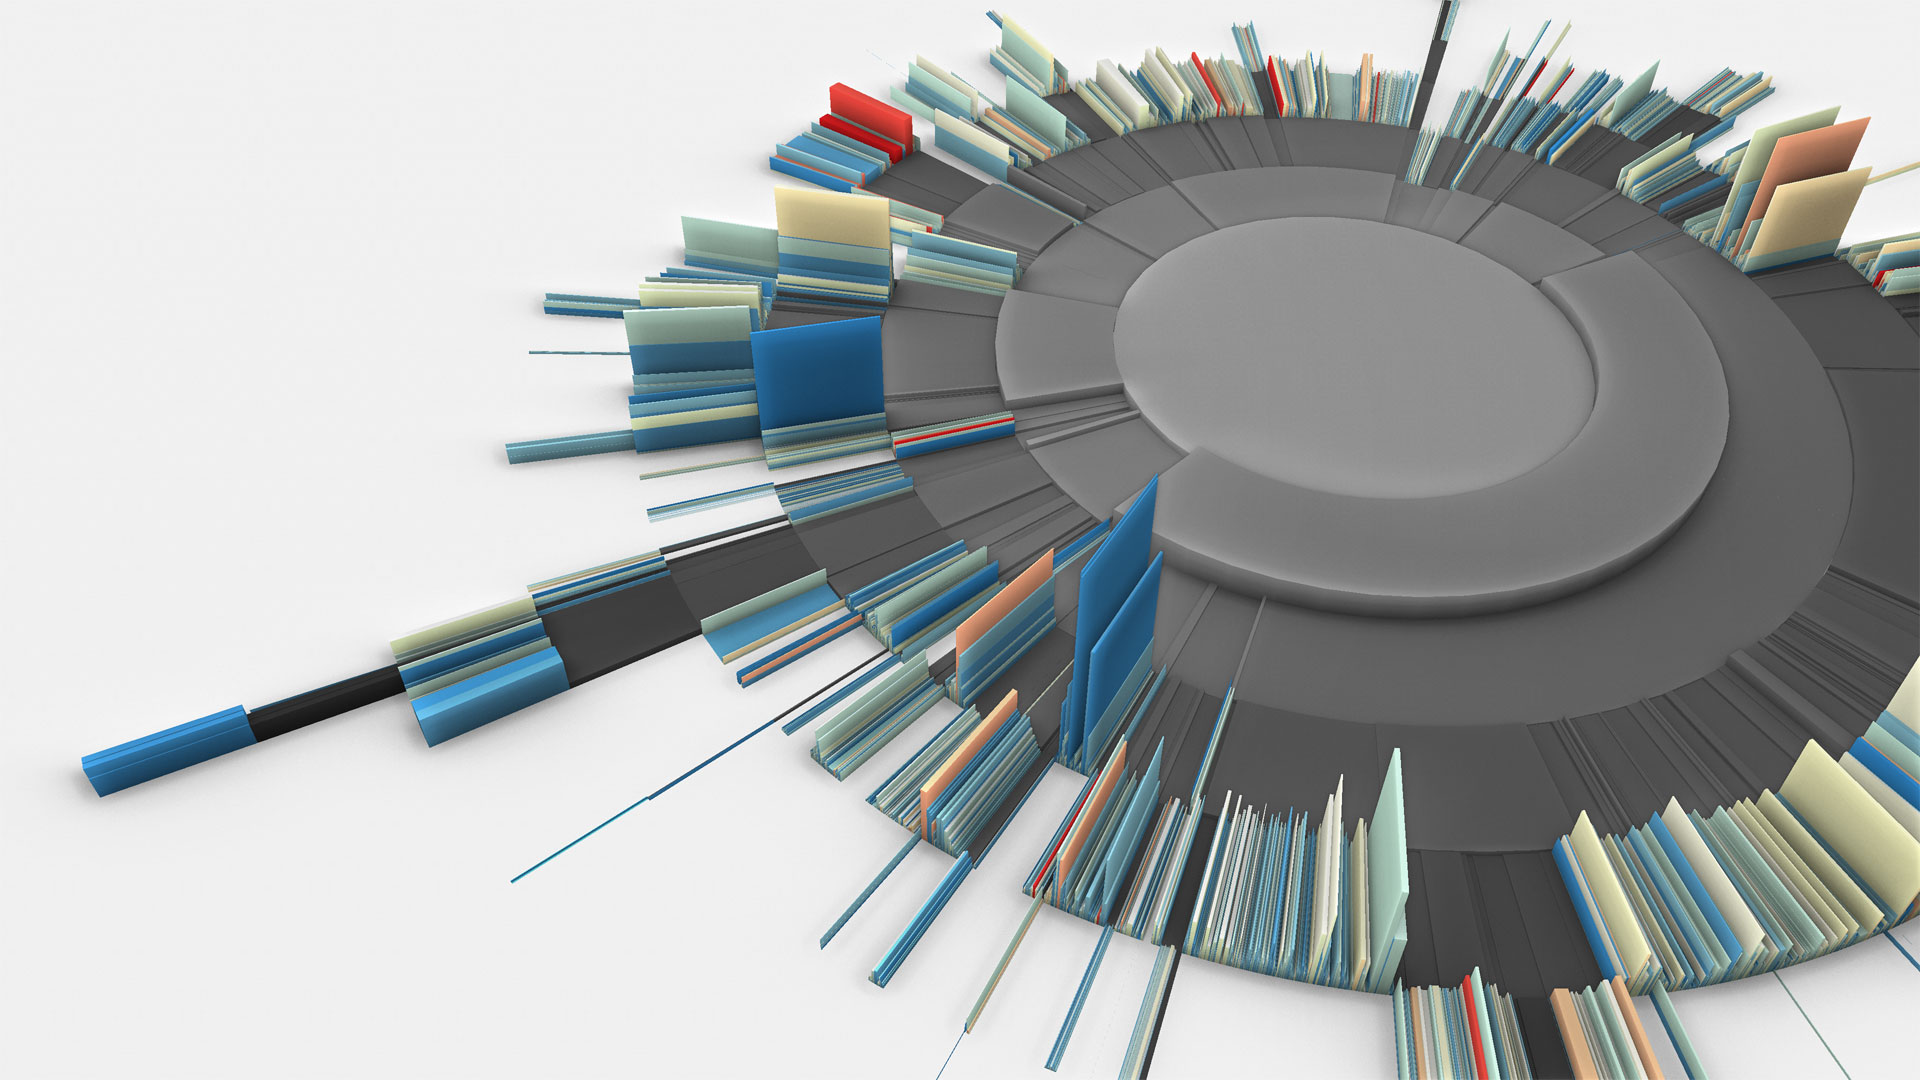
\includegraphics[width = \textwidth, clip, trim = 0 0 0 192]{figures/_sunburst_25d}};
    \end{tikzpicture}
    \caption{%
        An example of an adjacency layout for treemaps: a Sunburst view depicting a software system.}
    \label{fig:sunburst}
\end{figure*}
A prominent extension of software maps is adjacency layouts (\autoref{fig:sunburst}).
Most of them are derived from one-dimensional treemap layouts.
Using an extension to one dimension creates Icicle Plots and Flame Graphs~\citep{gregg2016-flamegraphs}, and a projection using polar coordinates results in Sunburst Views~\citep{stasko2000-structures} and Bundle Views~\citep{holten2006-edgebundles}.
Although a basic packing algorithm, the EvoStreets layout results in a software map using adjacency~\citep{steinbruckner2013-evolution}.
These layouts are convenient at the coarser levels of a software entity hierarchy, e.g., to display whole landscapes of software projects.
The nature of their layout allows for the explicit and complete depiction of inner nodes.
The additional whitespace can be used for additional mapping of inter-node relations~\citep{holten2006-edgebundles}.

\subsection{Layout Stability}
One of the biggest challenges for software maps is stability over time, i.e., node positions remain stable over time.
This is advantageous for the visual-data-correspondence~\citep{kindlmann2014-algebraic} and for maintaining a mental map~\citep{archambault2011-mentalmap}.
Stability is achieved by maintaining topology changes and weight changes of the underlying hierarchy.
Suppose the time range of interest is in the past. 
In that case, a multi-revision hierarchy can be computed~\citep{tu2007-changes}, allowing for stable positions of nodes as they can be pre-determined using a layout that incorporates all nodes with their maximum weight~\citep{pfahler2020-evolving}.
Suppose the software map is used to visualize ongoing processes and continuously evolving data. In that case, an initial layout can be incrementally evolved based on the topology changes, resulting in nodes growing, shrinking, appearing, and disappearing~\citep{scheibel2018-evocells}.
Moreover, \cite{kokash2014-templatebased} proposed an approach that ensures uniform treemap layouts over time by applying an explicit splitting scheme.
A similar approach is \emph{the layout of the treemap using only local modifications}~\citep{sondag2017-stabletreemaps} by applying local swaps and approximating the layout of the previous instance.
As an improvement to this, the Greedy Insertion approach operates on the derived layout tree and inserts new nodes next to the element with the worst aspect ratio~\citep{vernier2018-insertion}.

\section{Mapping}
\label{JOV:Sec:Mapping}
The mapping stage transforms pre-processed and filtered data, e.g., attribute values, into depictable and reversibly encoded graphical primitives and scenes.
This is a fundamental step for efficient encoding of input data and should address human capacities and abilities to decode a depiction~\citep{ware2012-information}.
There is not necessarily an explicit representation of the resulting visualization object in memory.
The result may only be volatile during visualization, especially from an implementation point of view: the distinction between mapping and rendering sustains more on a conceptual level~\citep{trapp2013-gputreemaps,scheibel2016-avcs}. 
In this section, visual variables and additional techniques available for attribute mapping are briefly described and discussed. 
An overview of visual variables (not techniques in general) is provided and summarized in \autoref{tab:overview-basic}. 
In it, each visual variable is classified with respect to the stage typically responsible as well as its applicability to (1) inner nodes and leaf nodes, (2) 2D and 2.5D software maps, and (3) the data type it most certainly can convey.


\begin{table*}[h]
  \centering
  \noindent%
  \renewcommand{\arraystretch}{1.25}
  \rowcolors{3}{white}{gray!15}%
  \setlength{\tabcolsep}{6pt}%
  \setlength{\aboverulesep}{14pt}%
  \setlength{\belowrulesep}{14pt}% 
  \setlength{\arrayrulewidth}{0.5pt}%
    \begin{tabular}{ r | c | c !{\tls} c | c !{\tls} c | c !{\tls} c !{\tls} c !{\tls} c }
      \multicolumn{1}{ c|}{\hspace{26mm}\textbf{Visual Variable}} & 
      \multicolumn{1}{ c|}{}     & 
      \multicolumn{2}{ c|}{Node}      & 
      \multicolumn{2}{ c|}{Dim.}      &
      \multicolumn{4}{ c }{Data Type} \\
      \rott{\strut \hspace{5em}} %
            &  \rott{\strut Stage} & \rott{\strut Inner Node} & \rott{\strut Leaf Node} 
            &  \rott{\strut 2D} & \rott{\strut 2.5D}  
            &  \rott{\strut Nominal} & \rott{\strut Ordinal} & \rott{\strut Interval} & \rott{\strut Ratio} \\\hline
      Area (Foot Print, Size)   & M   &   \OK & \OK &   \OK & \OK &       & \OK & \pa & \OK \\
      Color                     & R   &   \OK & \OK &   \OK & \OK &   \OK & \OK & \OK & \OK \\
      Height                    & M   &   \pa & \OK &       & \OK &       & \pa & \pa & \OK \\
      Transparency              & R   &   \pa & \OK &       & \OK &   \pa & \pa & \pa & \OK \\
      Light Emission (Glow)     & R   &   \pa & \OK &   \pa & \OK &       & \pa & \pa & \OK \\
      Stacking                  & M   &       & \OK &   \OK & \OK &   \OK &     & \pa & \OK \\
      Stacking (global layer)   & M   &   \pa & \OK &       & \OK &       & \pa & \pa & \OK \\
      Segments                  & M   &   \pa & \OK &   \OK & \OK &   \OK & \pa & \pa & \OK \\
      Shape Type                & M   &       & \OK &   \OK & \OK &   \OK & \pa &     &     \\
      Shape Parameter           & M   &   \pa & \OK &   \OK & \OK &       & \pa & \pa & \OK \\
      In-situ (Change, Diff)    & M   &       & \OK &   \OK & \OK &       & \OK &     &     \\
      Contour Width             & R   &   \OK & \OK &   \OK & \OK &       & \OK & \pa & \pa \\
      Contour Color             & R   &   \OK & \OK &   \OK & \OK &   \OK & \OK & \OK & \OK \\
      (Contour) Stippling       & R   &   \OK & \OK &   \OK & \OK &   \OK & \OK & \pa & \pa \\
      Sketchy Contour           & R   &   \OK & \OK &   \OK & \OK &   \pa & \OK & \pa & \pa \\
      Surface Pattern (Texture) & R   &   \pa & \OK &   \OK & \OK &   \OK & \OK & \pa & \pa \\
      Surface Noise (Texture)   & R   &   \pa & \OK &   \OK & \OK &   \pa & \OK & \pa & \OK \\
      Surface Shading (Texture) & R   &   \OK & \OK &   \pa & \OK &   \pa & \OK & \OK &     \\
      (Surface) Hatching        & R   &   \OK & \OK &   \OK & \OK &   \pa & \OK & \pa & \pa \\
      Nesting-Level Margin      & R   &   \OK &     &   \OK & \OK &       & \OK & \pa & \OK \\
      Color Weaving             & R   &   \OK & \OK &   \OK & \OK &   \OK & \pa &     &     \\
      Height Threshold          & R   &   \OK & \OK &   \OK & \OK &       & \pa & \pa & \OK \\\hline
  \end{tabular}%
  \caption{Legend: %
    M -- Mapping\enspace{}|\enspace{}R -- Rendering\enspace{}|\enspace{}\OK{} -- Supported\enspace{}|\enspace{}\pa{} -- Partially Supported %
  }
  \label{tab:overview-basic}%
\end{table*}%


\subsection{Use of Height}
\WrapFigRightRaised{figures/_swmap-using-height-cropped}{Using height as a visual variable by extruding the 2D shapes up (2.5D).}{fig:heightusage}
We utilize the height of cuboids by extrusion of the 2D shape~\citep{bladh2004-threedimensions,choi2011-stratatreemaps} as a secondary visual variable (\autoref{fig:heightusage}).
The idea is to convey information in the order of decreasing importance for the task: (1) color, (2) height, and (3) other visual variables.
For 2.5D software maps, pyramid-like shapes can be used to further encode an attribute or reduce occlusion~\citep{turo1992-improve}.
When depicting evolving data with accustomed map themes, height seems to allow for an intuitive encoding of data changes by means of growing or increasing vs. shrinking or decreasing, respectively.
Height, however, should not be used to depict negative or diverging scales directly, as this would result in downwards-facing cuboids.
Although suggested several times, we prefer to refine the map theme to transform or map relevant ranges of values of attributes to make a salient but expected use of visual variables: cuboids are high when the underlying data is interesting.
In contrast to that, if a negative value range is relevant, it is mapped inversely to height. 
If positive values are relevant, the absolute value could be mapped to height and the sign to color, shape, or texture.
Finally, the orientation of the leaf node's geometry~\citep{langelier2005-qualityanalysis} and the type, employing poly cylinders~\citep{marcus2003-softvis} and three-dimensional glyphs~\citep{boccuzzo2007-cognitive} are further suitable as visual variables.

\subsection{Juxtaposing and Complex Shapes}
For a visual display of multiple states or sub-elements, data vases, stacked cuboids, or segmenting/fragmenting can be used.
In remembrance of stacked bar charts, the extruded polytopes can be subdivided in height, allowing for the depiction of subcategories and their share of the overall height \citep{itoh2006-networkintrusion,giereth2008-patentportfolios}.
This process can further be utilized, \eg to encode evolution using \emph{evolution segments} \citep{steinbruckner2013-evolution} and \emph{data vases} \citep{thakur2009-datavases}.
Small multiples can be used for \enquote{the comparison of multiple software map themes and revisions simultaneously on a single screen} \citep{scheibel2016-smallmultiples}.
We found this especially useful for the generation of an overview as well as exploration and identification of map theme variations for software map assembly.

\subsection{Mixed Projections}
\WrapFigRightRaised{figures/_future-ortho-histo}{Inner node tilted into 2.5D (mixed projection) combined with a local histogram.}{fig:mixedprojections}
Recently, an approach for focus-sensitive use of 2D and 2.5D treemaps was presented. %
\enquote{The technique operates by tilting the graphical elements representing inner nodes using affine transformations and animated state transitions}~\citep{limberger2017-mixed}.
This allows for on-demand separation of high-detail focus areas and context areas (\autoref{fig:mixedprojections}).
It further reduces occlusion issues---which might occur for a particular data set or map theme---and the complexity of navigation.
Whenever occlusion becomes an issue, this usually hints at an inappropriate scaling, camera angle, or suboptimal map theme specification.
In almost all cases, occlusion issues can be resolved by applying simple mitigation strategies.

For software analytics, mixed projection can facilitate communication of the source code modules that target change for the current sprint.
In this example, the context is the other source code files present in the project.
Similarly, mixed projection can be used if the height mapping is irrelevant for the context but highly relevant for focus, e.g., using the estimated time to invest for a source code module to be mapped on height. 
Another technique to combine aggregated and detailed views with reduced occlusion is the \emph{lifted map}~\citep{chaudhuri2009-selfadaptive}.

\subsection{Depicting Change}
\WrapFigRightRaised{figures/_vv-in-situ}{In-situ template depicting changes in height.}{fig:insitu}
\begin{figure*}[b]
	\centering
	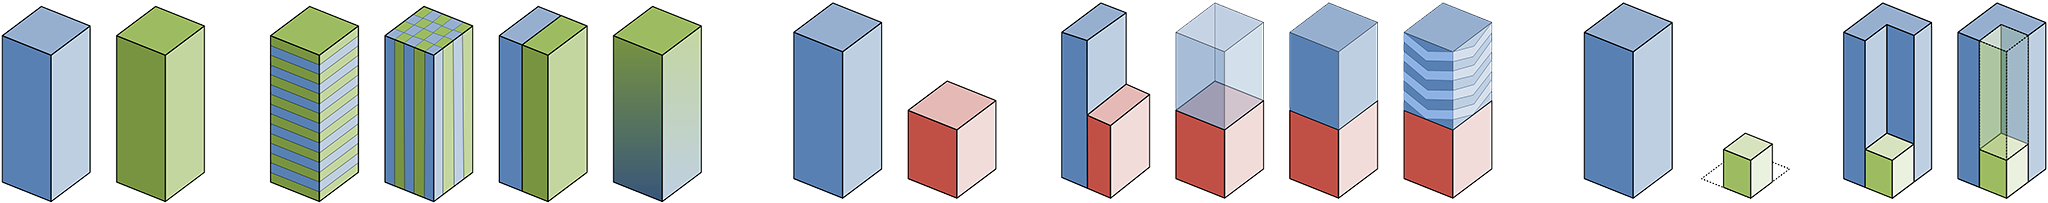
\includegraphics[width=\textwidth]{figures/_in-situ-templates}
	\caption{A set of in-situ templates to depict changes of up to three attributes using three or more visual variables \citep{limberger2019-insitu}.
		Left: templates for color-only changes. Middle: templates for color and height changes. Right: templates for changes in all area, height, and color.}
	\label{fig:insitu-templates}
\end{figure*}
Many software map themes are designed to facilitate understanding of the evolution of the underlying data sets (\autoref{fig:insitu}).
This eventually requires the visual comparison of (1) multiple visual variables for (2) multiple points in time over (3) large time ranges.
Therefore, \cite{tu2007-changes} introduced contrast treemaps.
Their approach could be applied within visual software analytics by encoding two different states of the attribute mapped to area and color.
This idea was extended by in-situ templates~\citep{limberger2019-insitu}, which allow for the visual encoding of former and latter states on a per-cuboid basis for rectangular 2.5D software maps~(\cf~\autoref{fig:insitu-templates}).
Specifically, basic and more complex templates were introduced to simultaneously depict changes in more than one visual variable, including area, color, and height.
Although not discussed in the paper, the templates allow for the comparison of additional per-node visual variables as well.
The visual quality and expressiveness thereby depend on the available rendering techniques, e.g., procedural texturing and transparency are accounted for by several templates~\citep{limberger2021-procedural-textures}.

In practice, most comparison templates would result in a complex mapping and should be used for complex tasks or expert systems only.
For example, depicting area changes in combination with others is challenging to perceive.
However, they allow for a convenient encoding of changes in height that are usually mapped from secondary information such as the number of authors or the size of domain logic.
Another use is to depict changes in color for preliminary information, i.e., the most prominent indicator for the primary purpose of the map theme, such as the maintainability or faultiness of a software module.

\subsection{Depicting Relations}
\WrapFigRightRaised{figures/_vv-relations}{Modules included by another module are connected using directed tubes (textured with procedurally generated arrows) in 3D.}{fig:relations}
For an emphasis on the topology with respect to the nested structure of nodes, cushion shading~\citep{vanwijk1999-cushion} or hierarchical stippling~\citep{sondag2020-uncertainty}, variations of margins or padding, as well as extruded, stacked inner nodes~\citep{bladh2004-threedimensions} can be applied.
If other relations (e.g., \autoref{fig:relations}) of nodes in addition to their tree-structured topology are of interest (e.g., functional dependencies or often-coinciding changes during the development process), edges or edge bundles can be superimposed onto software maps~\citep{holten2006-edgebundles,steinbeck2019-evostreets}.
This approach, however, is visually constrained by the number of depicted relations and data set size.
Superimposing relations using tubes on top of 2.5D treemaps introduces additional clutter and visual complexity not inherent to the treemap metaphor.

\section{Rendering}
\label{JOV:Sec:Rendering}
In this stage, the visualization object is transformed into images using (real-time) image synthesis. 
Although the mapping stage is usually aware of the available visual variables and metaphors, it only provides appropriate attribute values, descriptions of graphic primitives, and additional data for rendering.
As a result of the rendering stage, the mapped attributes should be visually encoded in the output image.

\subsection{Utilizing Texture Patterns}
\WrapFigRightRaised[-1.5]{figures/_vv-pattern}{Top faces textured with patterns (nominal mapping).}{fig:textures}
Different texture patterns can be applied to encode categorical data~\citep{molli2001-multisynchronous} (\autoref{fig:textures}).
Exemplary attributes for texture pattern mapping are (the abstract) file type (e.g., source code, documentation, deployment), associated teams, or budgets.
Alternatively, texture intensity was suggested as a visual variable for scales with a natural zero~\citep{holten2005-realism}.
With most modern rendering engines supporting physically based materials, textures can be used to enable visual variables based on their metalness or roughness (see natural metaphors).
In the past, we predominantly used procedural textures to depict quality measures (e.g., degree of documentation, error-proneness), complexity measures (incoming or outgoing dependencies, mixed-use of third-party dependencies), and development process indicators (e.g., number of authors). 
Procedural texturing can further be used to superimpose rulers or stripes, making the height effectively countable and increasing the accuracy of comparability.
Another approach is to use procedural textures to encode underlying data distributions~\citep{limberger2020-uncertainty}.

\subsection{Utilizing Emissive Light}
\WrapFigRightRaised{figures/_vv-emissive}{Emissive light (glow) as a visual variable in 2.5D.}{fig:emissivelight}
Emissive lighting can be an intuitive metaphor for activity:
if something lights up, something is going on (\autoref{fig:emissivelight}).
We used this to display development activity, e.g., through commits per day or the number of issues referencing a module. 
This visual variable can also be used to emphasize (highlight) nodes due to user interactions such as filtering and selection or to highlight system activity~\citep{dashuber2021-tracemaps}. 
However, today's real-time rendering systems are often incapable of rendering convincing light emissions, making this visual variable challenging to use.

\subsection{Using Sketchy Rendering}
\WrapFigRightRaised{figures/_vv-sketchy}{Sketchy outlines and hatching to depict uncertainty.}{fig:sketchiness}
For the visual display of uncertainty, fuzzy drawing styles can be applied.
For example, node contour width, as well as multiplexed frequency and amplitude, could be parameterized~\citep{gortler2017-bubbletreemaps} and used to indicate vagueness.
In addition, pencil-like outlines and hatching of surfaces can be combined into a single visual variable, i.e., \emph{sketchiness}.
Mapping data to sketchiness is instrumental in encoding \enquote{uncertainty, imprecision, or vagueness}~\citep{limberger2016-sketchy}.
It allows encoding varying degrees of uncertainty and can be used in addition to color (\autoref{fig:sketchiness}).
For example, it can display measurement inaccuracies (incomplete or estimated data) or target data that is yet to be discussed or implemented (i.e., targets for complexity, coverage, performance, or other quality measures).

\subsection{Utilizing Transparency}
\WrapFigRightRaised[-2.0]{figures/_vv-transparency-v2}{Transparency (stochastic) as a visual variable in 2.5D.}{fig:transparency}
Regarding geometric processing of inner nodes, some approaches extrude the layout as well, creating platforms~\citep{andrews1995-informationlandscapes} or pyramid frustums~\citep{andrews2002-informationpyramids}, and placing child nodes \emph{on top} of the platforms.
Instead of stacking, there are approaches for nested depiction as well, e.g., full spheres~\citep{balzer2004-softwarelandscapes} and hemispheres~\citep{balzer2004-largesoftware} in combination with transparency.
Other uses of transparency are (1) to reduce occlusion and (2) to encode different node states~\citep{luboschik2008-discovering}.
Transparency can further be used to depict removed or planned components, goals, and irrelevant nodes or enhance the expressiveness and quality of texturing (\autoref{fig:transparency}).
The most relevant obstacle to using transparency is its implementation complexity: especially for web-based rendering clients, modern strategies such as order-independent transparency cannot easily be implemented due to limited graphics APIs and device capabilities.
One solution is to use stochastic dithering combined with multi-frame sampling~\citep{limberger2017-highqualityrendering}.

\subsection{Depicting Aggregates and Structure}
\WrapFigRightRaised{figures/_at-aggregation}{Aggregation and nesting-level contours in a 2D treemap.}{fig:aggregates}
As previously discussed for the preprocessing and filtering stages, aggregation is an essential technique for software maps (\cf~\autoref{fig:aggregates}).
In the context of rendering, we suggest adhering to aggregation guidelines~\citep{elmqvist2010-aggregation}.
For example, the depiction should discern leaf nodes from aggregated ones.
In addition, small charts, diagrams, or glyphs encoding information of the underlying data can be expressed on top or within aggregates~\citep{soares2020-treemapglyphs}.
Likewise, noise or color weaving~\citep{haghshenas2007-colorweaving} as well as nesting-level contours---multiple contours that hint at the depth of the aggregated sub-tree, i.e., the number of an aggregate's subjacent hierarchy levels---can be used as well~\citep{limberger2017-aggregation}.
The aggregation should summarize contextual data of low variation for software maps to provide orientation without distraction.
Aggregation can further extend user control and interaction, e.g., folding and unfolding, as well as dynamically scaling the rendering load to comply with performance constraints.

\subsection{Height-based Filtering}
\WrapFigRightRaised{figures/_vv-ref-surface}{Reference surface for height-based filtering in 2.5D.}{fig:referencesurface}
For 2.5D software maps, a reference surface, a height reference~(\autoref{fig:referencesurface}) can be used to \enquote{facilitate accurate identification of highest nodes as well as similar nodes~[\ldots]. Furthermore, it allows filtering and selection of nodes based on their height and depicts filtered and unselected nodes in a clean way without introducing additional visual clutter}~\citep{limberger2018-filtering}.
Depending on the renderer's capabilities and the already occupied visual variables, one of the various approaches for the visual display of the height reference can be applied, e.g., intersection, stilts, explicit surface, closed surface, and implicit surface. %
Using user-induced aggregation (by means of folding and unfolding) in combination with an interactive height reference can provide a sufficient foundation for exploration-heavy tasks and map themes for single software maps and whole software map landscapes.

\subsection{Using Natural Metaphors}
\WrapFigRightRaised{figures/_vv-natural-metaphors}{Surface condition (rusty, shiny) as a visual variable.}{fig:naturalmetaphors}
Natural metaphors are based on the idea that \enquote{when faced with unfamiliar concepts, our cognitive system searches for the best mapping between the unknown concept and existing knowledge of other domains}~\citep{zhang2008-metaphors}.
To this end, natural metaphors, such as physically based materials (e.g., rust, radiant emittance, roughness, and shininess; \autoref{fig:naturalmetaphors}) or weather phenomena (e.g., rain, clouds, fire, dust, snow) were suggested to \enquote{emotionalize the visual communication by providing memorable visualizations} \citep{wurfel2016-naturalphenomena}.
These metaphors can be used to depict change predictions or deviations from expected values on a secondary visual variable while considering knowledge or best practices on preattentive processing of, e.g., numerical information~\citep{few2004-tapping,hesse2017-preattentive}.
However, weather phenomena require sophisticated rendering techniques, renderers, and an interactive context.
Further, their use might be inappropriate in certain professional contexts and even distracting for the map theme.

\section{Configuration of Software Maps}
\label{JOV:Sec:Configuration}
When assembling use-case-specific map themes, implementation and provisioning have to be considered.
For example, most visual variables have to be tweaked for the actual screen size, pixel density, and number or average size of nodes. 
In addition, all visual variables used have to be (re)adjusted within the context of their specific combination and their intended task. 
A few general remarks are provided in the following, which can be considered regardless of the specific visual variables used to assemble more effective map themes.

\subsection{Labeling and Text}
\WrapFigRightRaised{figures/_at-labeling}{Enhancing treemaps using dynamic text placement.}{fig:labeling}
More than twenty years ago, \citeauthor{fekete1999-labeling} stated that \enquote{a major limiting factor to the widespread use of information visualization is the difficulty of labeling information abundant displays}~\citep{fekete1999-labeling}. 
At the time of writing, this is still a \enquote{major limiting factor} today in most visualizations.
Different techniques that augment treemaps with text have been proposed and evaluated for treemaps.
The prominent approach is the usage of the nodes' surface to integrate labels in terms of \emph{internal annotations}~\citep{limberger2017-aggregation} (\autoref{fig:labeling}).
This approach usually affects the layout computation if applied to inner nodes as well \citep{liu2008-nsffunding}.
The complementary approach, \emph{external labeling}, is not treemap-specific but induces common problems such as \enquote{overlaps and data occlusion}~\citep{fekete1999-labeling}.
Typically, external labels are positioned as hovered text in proximity to its node~\citep{slingsby2008-variableselection} or a connected line to indicate association \citep{bladh2004-threedimensions}.
Additionally, the size of the label may be used to encode importance~\citep{jadeja2017-graphlabeling}.

One challenge remains: Integrating techniques that allow for dynamic, interactive, adaptive, and high-quality text display in 3D scenes. 
To this end, the Open Label Library (OpenLL) project is an essential step toward a low-level, implementation-aware specification for dynamic, hardware-accelerated rendering and smart, adaptive placement of text~\citep{limberger2017-openll}.
Users should be allowed to not only read a text but select, copy and paste, and change within their 3D visualization. 

\subsection{Visual Cues}
Visual cues can increase the effectiveness of visualization.
They can be associated with certain visual variables to convey information either more effectively or at all.
Apart from that, visual cues can be added to the visual variables used. 
Shadows, cushion shading, paddings and margins, or shading, for example, can significantly impact the readability of software maps.
For example, a 2.5D treemap that does not employ padding or some form of lighting or shading will be much harder to read. 
Likewise, missing shadows or outlines can make it hard to perceive the topology or differentiate individual nodes from one another.
At the same time, it is not necessarily helpful for the rendering to strive for as much realism as possible since this often can cause visual clutter (e.g., the use of reflections can be somewhat distracting).
In any case, the visual cues should be adjusted carefully to the map theme.
The combined use of information visualization and visual cues with a claim to reality is an open field in research.

\begin{figure*}[t] %
    \begin{tikzpicture}[figNS, spy using outlines = {style = spyRC, magnification = 2.0, width = 20mm, height = 20mm}]
        \node[figRC, anchor = east](fig0) at (0,0)
            {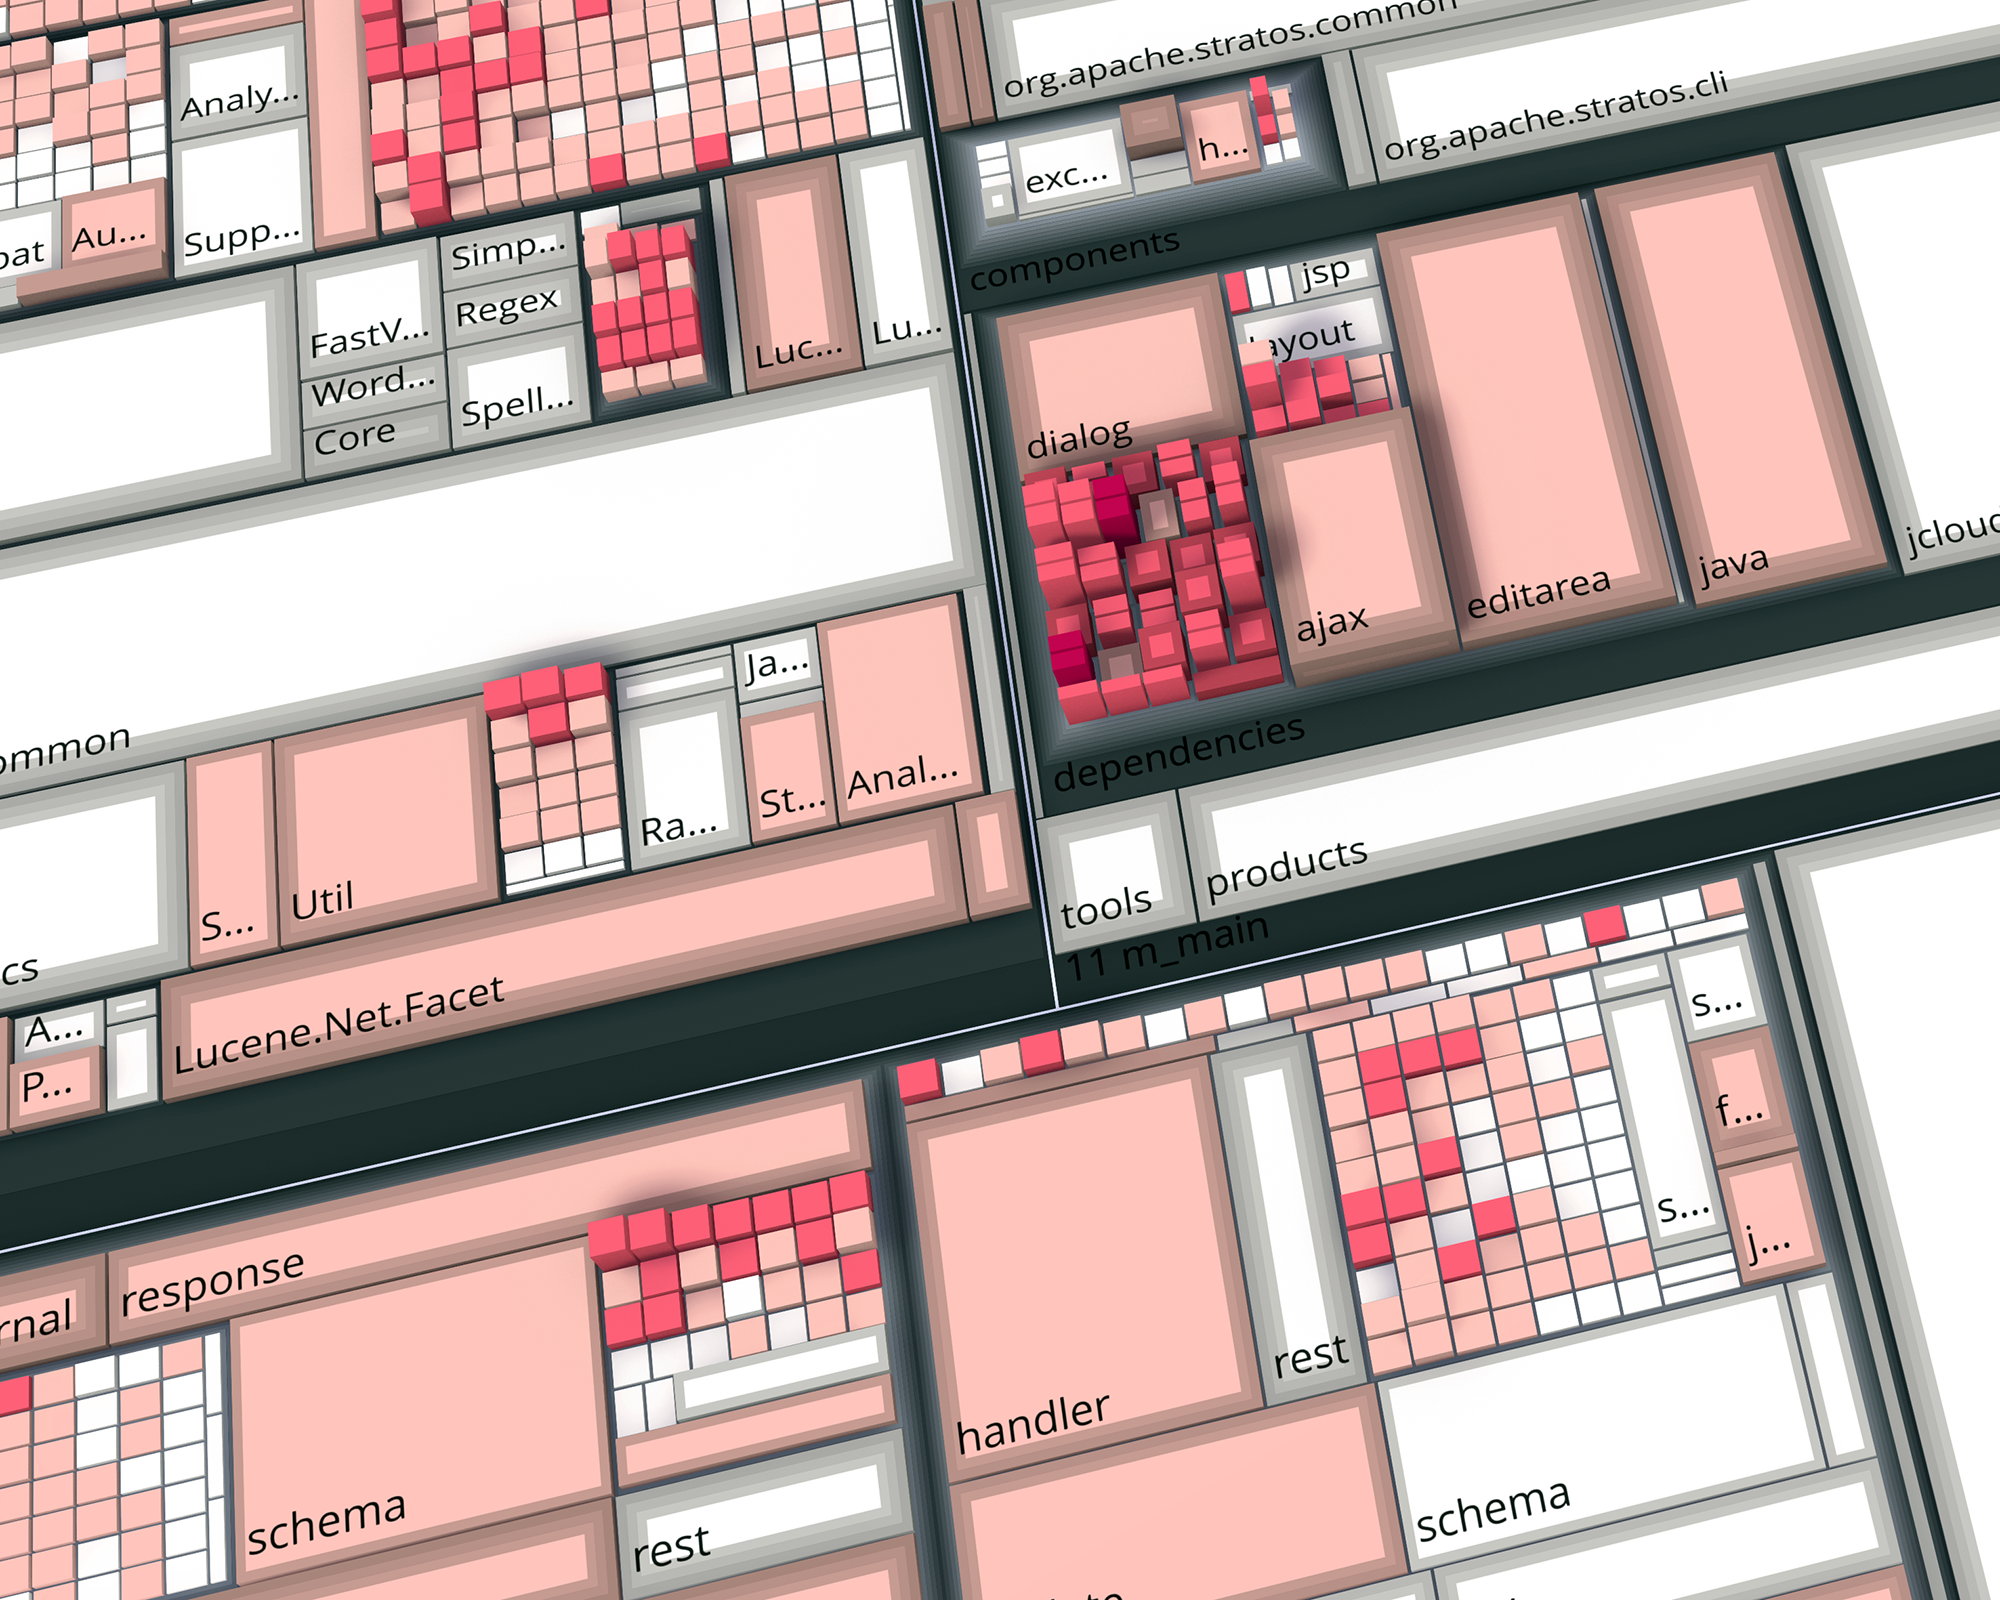
\includegraphics[width = \twffp, trim = 0 0 0 0, clip]{figures/_aggregated-25d}};
        \node[figRC, anchor = west](fig1) at ([xshift = \pfull] fig0.east) 
            {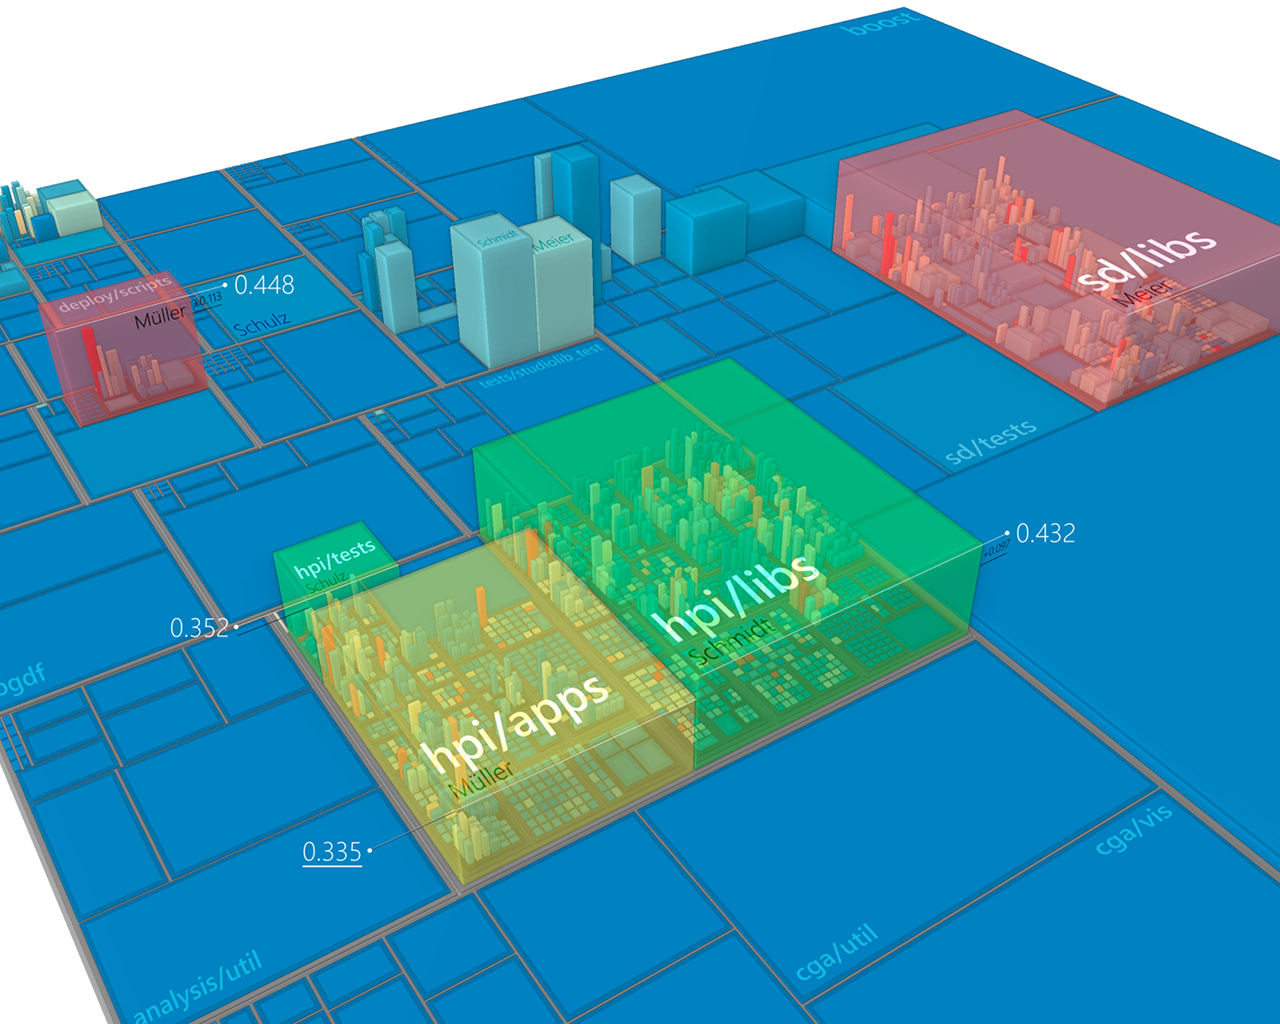
\includegraphics[width = \twffp, trim = 0 0 0 0, clip]{figures/_multi-semantic-treemap-cropped}};
        \node[below left = 0 of fig0, labelSW](lab0){(a)};
        \node[below left = 0 of fig1, labelSW](lab1){(b)};
        \spy on ($(fig0.center)+(-14mm, +14mm)$) in node at ($(fig0.north)+(+16mm,-13mm)$);
        \spy on ($(fig1.center)+(-20mm, +8mm)$) in node at ($(fig1.north)+(+16mm,-13mm)$);
    \end{tikzpicture}
    \caption{%
        Two examples of complex software map assemblies: (a) aggregation and internal labeling \citep{limberger2017-aggregation}.
        The resulting space from aggregating nodes is used to embed labels into the software map. And (b) a semi-transparent information overlay to superimpose and emphasize additional information.}
    \label{fig:complex-examples}
\end{figure*}

\subsection{Assembling Treemaps}
\begin{table*}[t]
  
\centering
\small
\noindent%
\renewcommand{\arraystretch}{1.25}
\rowcolors{2}{white}{gray!15}%
\setlength{\tabcolsep}{1pt}%
\setlength{\aboverulesep}{14pt}%
\setlength{\belowrulesep}{14pt}% 
\setlength{\arrayrulewidth}{0.5pt}%
\begin{tabular}{r | c !{\tls} %
  c !{\tls} c !{\tls} c !{\tls} c !{\tls} c !{\tls} %
  c !{\tls} c !{\tls} c !{\tls} c !{\tls} c !{\tls} %
  c !{\tls} c !{\tls} c !{\tls} c !{\tls} c !{\tls} %
  c !{\tls} c !{\tls} c !{\tls} c !{\tls} c !{\tls} %
  c}
    \rott{\strut \hspace{9.5em}} %
  & \rott{\strut Area} 
  & \rott{\strut Color} 
  & \rott{\strut Height} 
  & \rott{\strut Transparency} 
  & \rott{\strut Light Emission} 
  & \rott{\strut Stacking}  
  & \rott{\strut Stacking (global layer)} 
  & \rott{\strut Segments} 
  & \rott{\strut Shape Type} 
  & \rott{\strut Shape Parameter} 
  & \rott{\strut In-situ} 
  & \rott{\strut Contour Width} 
  & \rott{\strut Contour Color} 
  & \rott{\strut Stippling} 
  & \rott{\strut Sketchy Contour} 
  & \rott{\strut Pattern} 
  & \rott{\strut Noise} 
  & \rott{\strut Shading} 
  & \rott{\strut Hatching} 
  & \rott{\strut Nesting-Level Margin} 
  & \rott{\strut Color Weaving} 
  & \rott{\strut Height Threshold} 
  \\\hline
  Area (Foot Print, Size) & --  &     &     &     &     &     &     &     &     &     &     &     &     &     &     &     &     &     &     &     &     &    \\
  Color                   & \OK & --  &     &     &     &     &     &     &     &     &     &     &     &     &     &     &     &     &     &     &     &    \\
  Height                  & \OK & \OK & --  &     &     &     &     &     &     &     &     &     &     &     &     &     &     &     &     &     &     &    \\
  Transparency            & \OK & \pa & \OK & --  &     &     &     &     &     &     &     &     &     &     &     &     &     &     &     &     &     &    \\
  Light Emission (Glow)   & \OK & \pa & \OK & \pa & --  &     &     &     &     &     &     &     &     &     &     &     &     &     &     &     &     &    \\
  Stacking                & \OK & \OK & \OK & \OK & \OK & --  &     &     &     &     &     &     &     &     &     &     &     &     &     &     &     &    \\
  Stacking (global layer) & \OK & \OK & \OK & \OK & \OK &     & --  &     &     &     &     &     &     &     &     &     &     &     &     &     &     &    \\
  Segments                & \OK & \OK & \OK & \OK & \OK & \OK & \OK & --  &     &     &     &     &     &     &     &     &     &     &     &     &     &    \\
  Shape Type              & \OK & \OK & \OK & \OK & \pa & \pa & \pa & \pa & --  &     &     &     &     &     &     &     &     &     &     &     &     &    \\
  Shape Parameter         & \OK & \OK & \OK & \OK & \OK & \pa & \pa & \pa &     & --  &     &     &     &     &     &     &     &     &     &     &     &    \\
  In-situ (Change, Diff)  & \OK & \OK & \OK & \OK & \OK &     &     & \pa & \pa & \pa & --  &     &     &     &     &     &     &     &     &     &     &    \\
  Contour Width           & \OK & \OK & \OK & \pa & \pa & \OK & \OK & \pa & \pa & \pa & \pa & --  &     &     &     &     &     &     &     &     &     &    \\
  Contour Color           & \OK & \pa & \OK & \pa & \pa & \OK & \OK & \OK & \pa & \pa & \pa & \OK & --  &     &     &     &     &     &     &     &     &    \\
  (Contour) Stippling     & \OK & \pa & \OK & \pa & \pa & \OK & \OK & \pa & \pa & \pa & \pa & \OK & \OK & --  &     &     &     &     &     &     &     &    \\
  Sketchy Contour         & \OK & \OK & \OK & \pa & \pa & \OK & \OK & \pa & \pa & \pa & \pa & \OK & \pa & \pa & --  &     &     &     &     &     &     &    \\
  Surface Pattern         & \OK & \OK & \OK & \pa & \pa & \OK & \OK & \OK & \OK & \OK & \pa & \OK & \OK & \pa & \pa & --  &     &     &     &     &     &    \\
  Surface Noise           & \OK & \OK & \OK & \pa & \pa & \OK & \OK & \OK & \OK & \OK & \pa & \OK & \OK & \pa & \pa &     & --  &     &     &     &     &    \\
  Surface Shading         & \OK & \OK & \OK & \pa & \pa & \OK & \OK & \pa & \OK & \OK & \pa & \OK & \OK & \OK & \pa & \pa & \pa & --  &     &     &     &    \\
  (Surface) Hatching      & \OK & \OK & \OK & \pa & \pa & \OK & \OK & \OK & \OK & \OK & \pa & \OK & \OK & \pa & \OK &     &     &     & --  &     &     &    \\
  Nesting-Level Margin    & \OK & \pa & \OK & \pa & \pa & \OK & \OK &     & \pa &     &     &     &     &     &     & \OK & \OK & \OK & \OK & --  &     &    \\
  Color Weaving           & \OK & \pa & \OK & \pa & \pa & \pa & \OK & \OK & \OK & \OK & \pa & \pa & \pa & \pa & \pa & \pa &     &     &     & \pa & --  &    \\
  Height Threshold        & \OK & \OK & \OK & \pa & \OK &     &     &     & \pa & \pa & \pa & \OK & \OK & \OK & \pa & \OK & \OK & \OK & \OK &     & \OK & -- \\
  \hline
\end{tabular}%


  \caption{%
    This is-combinable-with matrix is symmetric. 
    The data is based on the authors' assessment. 
    Simultaneous use of four or more visual variables, however, should always be carefully considered regardless of their technical compatibility.
    Legend: \OK{} -- well combinable\enspace{}|\enspace{}\pa{} -- difficult to combine.}
  \label{tab:overview-assembly}%
\end{table*}%

When assembling a map theme, we usually gather all input characteristics (data types, data resolution, etc.) and specify the use case(s) and related tasks as clearly as possible.
The resulting software maps differ in their used metaphors and visual variables (\autoref{fig:complex-examples}).
For example, does the task consist of stepwise exploration or subsequent queries that could be addressed within the visualization directly (overview+detail, primary and secondary concerns, or root cause analysis)?
Is the visualization part of a multiple-linked-view setup, preceded by other investigations, or part of a broader analytics process?
What are the time and frequency the user needs to complete the task or use the visualization, respectively?

In most cases, our software maps first and foremost assist the user in identifying regions or nodes of interest.
Then, additional visual variables are employed for subsequent exploration of the relevant data for those nodes.
Tables \ref{tab:overview-basic} and \ref{tab:overview-assembly} are intended to facilitate the identification of promising visual variables and combinations most appropriate for the task.
Whether or not the visual variables can be used depends most certainly on the limitations of the targeted devices and used frameworks. 
As stated before, transparency, emissive lighting, and similar, technically demanding visual variables are highly convenient but still hard to implement for interactive use.

\section{Conclusions}
\label{JOV:Sec:Conclusions}
This paper reviewed advanced visual metaphors and visualization techniques for software maps.
A brief discussion of each metaphor and technique is extended by common practices and own experiences by the authors.
Notably, the presented techniques are modular and can be used in combination in an on-demand manner without conflicting with other techniques.
This way, the software map can be used for a wide range of use cases.
The approaches can visually scale from small to large and even massive data sets and allow for mapping multiple attributes for data-driven decision-making.
To summarize, we argue that the software map is a highly versatile tool in visual software analytics.

For future work, we foremost acknowledge the current state of evaluation for treemaps and software maps~\citep{fiedler2020-treemap-evaluation}.
This motivates further evaluation of the proposed metaphors and techniques by means of user studies and studies in industry contexts.
Further, we want to evaluate the applicability of the advanced metaphors and techniques to other 2D and 2.5D information visualization techniques.
This includes visualization techniques from the classes of implicit edge representation trees and mapped trees for hierarchically structured software data~\citep{scheibel2020-treemaptaxonomy} and topic maps for unstructured or otherwise-structured software data~\citep{atzberger2021-softwareforest}.

\section*{Acknowledgments}
We want to thank the anonymous reviewers for their valuable comments and suggestions to improve this article.
This work is part of the \enquote{Software-DNA} project, which is funded by the European Regional Development Fund (ERDF or EFRE in German) and the State of Brandenburg (ILB).
This work is also part of the KMUi project \enquote{KnowhowAnalyzer} (01IS20088B), which is funded by the German Federal Ministry of Education and Research (BMBF), and
the ZIM project \enquote{TASAM}, which is funded by the German Federal Ministry for Economic Affairs and Energy (BMWi).

\bibliographystyle{spbasic}
\bibliography{references}

\end{document}
